\documentclass[mathematics,article,submit,pdftex,moreauthors]{Definitions/mdpi}

\usepackage{tikz}
\usepackage[ruled,vlined,linesnumbered]{algorithm2e}
\SetKwInput{KwData}{Input}
\SetKwInput{KwResult}{Output}
\usetikzlibrary{shapes,arrows.meta,positioning,calc,patterns,decorations.pathreplacing,shadows,fit,backgrounds}
\usepackage{subfig}
\usepackage{multirow}
\usepackage{booktabs}
\usepackage{microtype}
\renewcommand{\qedsymbol}{}

% === SHARED FIGURE COLOUR PALETTE (uniform across all figures) ===
% Identical hex values to the result figures (regen_figs_academic.py).
\definecolor{acBlueD}{HTML}{1F3B57}  % dark navy
\definecolor{acBlue}{HTML}{3B6EA5}   % mid blue
\definecolor{acBlueL}{HTML}{A6C5E3}  % light blue
\definecolor{acRed}{HTML}{C0392B}    % red accent (thresholds/feedback)
\definecolor{acGreen}{HTML}{4F8F5B}
\definecolor{acAmber}{HTML}{E0A338}
\definecolor{acMag}{HTML}{B5538A}
\definecolor{acGrey}{HTML}{6E7B8B}

% === TITLE AND AUTHORS ===
\Title{Uncertainty-Aware Temporal Convolutional Networks for Multivariate Anomaly Detection: A Composite-Objective Framework with Chebyshev Bounds}
% === AUTHORS ===

\newcommand{\orcidauthorA}{0000-0001-9790-7597}
\newcommand{\orcidauthorB}{0000-0003-1020-9628}
\newcommand{\orcidauthorC}{0000-0003-0466-8254}
\newcommand{\orcidauthorD}{0000-0003-2168-7983}
\newcommand{\orcidauthorE}{0000-0000-0000-0000}

\Author{Vandha Pradwiyasma Widartha $^{1}$\orcidA{}, Ifrina Nuritha $^{2}$\orcidB{}, Kyung Hyune Rhee $^{3}$\orcidC{}, Young Po Hwang $^{4}$\orcidE{} and Chang Soo Kim $^{1,}$*\orcidD{}}
\AuthorNames{Vandha Pradwiyasma Widartha, Ifrina Nuritha, Kyung Hyune Rhee, Young Po Hwang and Chang Soo Kim}

\address{%
$^{1}$ \quad Department of Information Systems, Pukyong National University, Busan 48513, Republic of Korea; vandhapw@pukyong.ac.kr\\
$^{2}$ \quad Department of Information System, University of Jember, Indonesia 68121, Republic of Indonesia; ifrinanuritha@unej.ac.id\\
$^{3}$ \quad Division of Computer Engineering and AI, Pukyong National University, Busan 48513, Republic of Korea; khrhee@pknu.ac.kr\\
$^{4}$ \quad Research Center, Hanyoung DS, Inc., Seoul, 07600, Republic of Korea; hyp6511@hyds.kr}
\corres{Correspondence: cskim@pknu.ac.kr}


% === ABSTRACT ===
\abstract{Multivariate time-series anomaly detection on physical sensor networks faces three challenges that generic deep learning models inadequately addressed: heterogeneous sensor reliability, context-dependent anomaly scoring, and inactionable binary outputs lacking per-sensor attribution. We propose an uncertainty-aware Temporal Convolutional Network (TCN) framework built on two tightly integrated uncertainty-driven components: (i) an Adaptive Uncertainty-Aware Attention (AUAA) mechanism that gates temporal attention weights by per-sensor predictive uncertainty obtained from Monte-Carlo dropout; and (ii) a Dynamic Weight Adapter that learns context-sensitive blending of reconstruction error and uncertainty via a GRU over weight history. The architecture also includes an exploratory per-sensor attribution head, which we audit rather than claim: a controlled-perturbation test shows it is not yet causally faithful, and we report this transparently as a limitation. We complement the empirical architecture with two distribution-free theoretical results: a Chebyshev-type false-positive bound on the hybrid anomaly score, and a Monte-Carlo posterior moment convergence result at rate $O(M^{-1/2})$. Evaluated on four-month indoor air quality sensor data, the Full Enhanced model achieves $R^{2}=0.9988$ and MSE $1.65\times 10^{-4}$, a $25.2\%$ MSE reduction over the Base TCN ($R^{2}=0.9984$, MSE $2.20\times 10^{-4}$). Cross-dataset validation on the Skoltech Anomaly Benchmark (SKAB) a publicly available labelled industrial water-circulation corpus disjoint from the IAQ training distribution yields a $7.7\times$ F1 advantage ($0.477$ vs.\ $0.062$) and a $12.6\times$ recall advantage ($0.418$ vs.\ $0.033$) for the proposed model configuration over the Base TCN at a validation-calibrated threshold applied without retuning; against twelve established detectors under a unified protocol it attains the best F1 and recall, while trading some precision. Ablation isolates each component's contribution, the detector degrades gracefully under channel masking and noise, and the distribution-free false-positive bound is empirically respected. The framework retains a low inference cost ($0.16$\,ms per window at $M=20$ Monte-Carlo samples, including the uncertainty pass).}

\keyword{multivariate time series; anomaly detection; temporal convolutional network; uncertainty quantification; Monte-Carlo dropout; adaptive attention; Chebyshev}

% === MDPI FRONT-MATTER METADATA (placeholder values for submission) ===
\firstpage{1}
\makeatletter
\setcounter{page}{\@firstpage}
\makeatother
\pubvolume{1}
\issuenum{1}
\articlenumber{0}
\pubyear{2026}
\copyrightyear{2026}
\datereceived{}
\daterevised{}
\dateaccepted{}
\datepublished{}

\begin{document}


% ============================================================
\section{Introduction}
Multivariate time-series data generated by sensor networks for environmental monitoring, industrial control, and building management embed critical operational intelligence and pose distinct analytical challenges that drive recent advances in time-series analysis~\cite{kumar2022iaq_review, szczurek2020iaq}. Among these challenges, anomaly detection on multivariate time series is a central problem with applications spanning fault diagnosis, structural health monitoring, and process safety. Indoor air quality (IAQ) monitoring exemplifies the multivariate sensor-stream regime: CO\textsubscript{2}, volatile organic compounds (VOC), temperature, humidity, and particulate matter exhibit complex co-variation patterns while each sensor type suffers from distinct noise characteristics, calibration drift rates, and failure modes~\cite{coleman_sensing_2018, abid2021iaq_deep}. Time-series anomaly detection has been extensively surveyed~\cite{chandola2009survey, aggarwal2017outlier, pang2021deep_survey}, with recent IAQ-specific studies leveraging deep architectures for both forecasting and outlier identification~\cite{choi2024air_anomaly, wei2023lstm_ae_iaq}. In practice, deployment necessitates solutions that confront challenges unique to physical sensor networks, situated within a mathematically rigorous time-series framework—challenges that conventional time-series models fail to explicitly address.

This study is motivated by three sensor-specific challenges. First, multi-sensor deployments exhibit heterogeneous reliability across time. Individual sensors degrade at different rates: electrochemical VOC sensors drift over weeks, optical dust sensors saturate in high-concentration events, and temperature sensors maintain stable calibration for months~\cite{sanchez-ferrera_review_2025}. Standard attention mechanisms treat all time steps equally, yet predictions for a degrading VOC sensor at time $t$ are inherently less reliable than predictions for a stable temperature sensor at the same instant. A sensor-aware model should dynamically down-weight attention to unreliable channels. Second, anomaly scoring must adapt to context. Most approaches combine reconstruction error and prediction uncertainty using fixed weights~\cite{ghimire_electricity_2025, cui_sde-hnn_2025}, but the relative informativeness of these signals depends on sensor state: during stable operation, large reconstruction errors reliably indicate anomalies; During degradation events, a high level of uncertainty may actually serve as a more reliable signal, even though reconstruction errors appear moderate. A fixed-weight scoring system combines these two distinct conditions, thereby reducing detection accuracy during sensor transitions. Third, anomaly detectors should produce actionable output. Binary flagging without sensor-level attribution leaves facility operators unable to determine whether a detected anomaly reflects a genuine environmental hazard, a degrading CO\textsubscript{2} sensor requiring recalibration, or a VOC spike from cleaning activities~\cite{xu2022anomalytransformer}. For anomaly detection to inform maintenance decisions, it must identify which sensors contribute to each anomaly and provide uncertainty-aware estimates rather than only point predictions.

The Temporal Convolutional Network (TCN) architecture~\cite{bai2018tcn} provides an effective backbone for sequence modeling through dilated causal convolutions, matching or exceeding recurrent models on time-series benchmarks. Monte Carlo (MC) dropout~\cite{gal2016dropout_bayesian} enables uncertainty estimation from deterministic architectures without requiring explicit Bayesian inference. Neither technique alone, however, addresses the sensor-specific challenges described above. The principal contribution of this study lies in the integration of uncertainty signals, not as independent outputs, but as internal mechanisms that actively influence attention computation, anomaly scoring, and sensor-level attribution, thereby aligning with the operational realities of physical sensor deployments.

We present an uncertainty-aware TCN framework for multivariate sensor anomaly detection, making three contributions tightly coupled to the challenges above:

\begin{enumerate}[leftmargin=*, nosep]
    \item \textbf{Adaptive Uncertainty-Aware Attention (AUAA).} An attention mechanism that modulates temporal attention weights using per-sensor predictive uncertainty estimates via an uncertainty gate $g_t = 1/(1 + \sigma_t)$. This makes attention computation sensitive to sensor-specific reliability fluctuations, enabling the model to down-weight unreliable channels.
    
    \item \textbf{Dynamic Weight Adapter for Hybrid Anomaly Scoring.} A learnable gating module that contextually balances reconstruction error against predictive uncertainty using a GRU over recent weight history. This replaces static combination weights with a mechanism that adapts to sensor operating conditions.
    
    \item \textbf{Feature-Level Anomaly Attribution with Theoretical Bounds.} A feature-importance learner providing per-sensor explanations, complemented by Chebyshev-based uncertainty bounds that guarantee $P(\text{false positive}) \leq 1/k^2$. This delivers actionable, sensor-specific explanations with provable calibration guarantees.
\end{enumerate}

% We validate through four-month IAQ sensor data, comprehensive ablation studies isolating each component, cross-dataset evaluation on the Skoltech Anomaly Benchmark (SKAB)~\cite{skab_dataset}.
% a publicly available labelled industrial water-circulation corpus whose ground-truth labels are exogenous to our model development pipeline and sensitivity analysis of key hyperparameters.

% ============================================================
\section{Related Works}

\subsection{Deep Anomaly Detection in Multivariate Time Series}

Multivariate time-series anomaly detection has evolved from classical statistical methods toward deep architectures that learn normal behavioural patterns and identify deviations~\cite{pang2021deep_survey}. Foundational sequence models LSTM~\cite{hochreiter1997lstm}, GRU~\cite{cho2014gru}, and the TCN~\cite{bai2018tcn} established the architectural vocabulary for temporal modelling. The TCN, in particular, demonstrated that dilated causal convolutions provide a competitive alternative to recurrence, with advantages in training stability and parallel computation. WaveNet~\cite{oord2016wavenet} originally introduced dilated causal convolutions for sequence modelling; subsequent comprehensive reviews~\cite{zhang2020tcn_review} catalogue the diverse extensions that have since been applied to industrial time series.

Recent work has extended TCNs with complementary techniques: TCN-AE architectures~\cite{thill_temporal_2021} leverage autoencoding for unsupervised detection; TCN-Linear hybrids~\cite{wang_tcn-linear_2024} combine convolutional and linear residual paths; and attention-augmented TCNs~\cite{mehta_nac-tcn_2023} incorporate self-attention for industrial monitoring applications. Reconstruction-based anomaly detectors such as USAD~\cite{audibert2020usad} and LSTM-ED~\cite{malhotra2016lstmed} learn normal-behaviour priors and threshold residuals at inference. Transformer-based detectors such as TranAD~\cite{tuli2022tranad} and Anomaly Transformer~\cite{xu2022anomalytransformer} introduce self-attention for anomaly scoring; recent designs (e.g., Informer~\cite{zhou2021informer}, TimesNet~\cite{wu2022timesnet}, MTAD-GAT~\cite{zhao2020mtadgat}) further enrich the attention vocabulary but do not incorporate predictive uncertainty into the attention mechanism itself.

Despite this progress, existing TCN-based detectors treat sensor readings as generic multivariate inputs without modelling sensor-specific reliability characteristics. Our work explicitly couples uncertainty estimation to attention computation and anomaly scoring, adapting model behaviour to the varying reliability of individual sensor channels. Uncertainty quantification (UQ) transforms anomaly detection from threshold-based heuristics into confidence-aware decisions~\cite{kendall2017uncertainties}. Dropout as a Bayesian approximation~\cite{gal2016dropout_bayesian} provides a lightweight mechanism for estimating predictive uncertainty from deterministic architectures, building on the original dropout regularizer~\cite{srivastava2014dropout}; deep ensembles~\cite{lakshminarayanan2017ensembles} offer an alternative with stronger calibration at higher computational cost. MC dropout has been validated across diverse time-series domains: electricity demand forecasting with TCNs~\cite{ghimire_electricity_2025}, stochastic differential equation-based hydrological forecasting~\cite{cui_sde-hnn_2025}, and multivariate imputation. These works demonstrate that MC dropout provides meaningful uncertainty estimates, but they apply uncertainty post hoc as a separate scoring term rather than feeding it back into the model's internal representations. Our framework advances this field of study by closing the loop: uncertainty estimates modulate attention weights and condition the dynamic scoring function, creating integration between UQ and model computation motivated by sensor-specific reliability concerns.

For attention mechanisms in temporal data, the Transformer's self-attention~\cite{vaswani2017attention} enables the direct calculation of relationships between tokens and captures long-range dependencies that might be missed by convolutional filters. Standard attention assumes all input positions are equally trustworthy an assumption violated by physical sensor data where individual measurements carry sensor-specific uncertainty. Conformal prediction~\cite{angelopoulos2021conformal} and concentration-inequality machinery~\cite{boucheron2013concentration} provide distribution-free statistical guarantees, but operate at the output level rather than altering internal representations. Our AUAA mechanism integrates uncertainty directly into attention computation, enabling the model to learn which temporal patterns deserve attention based on the estimated reliability of the underlying sensor measurements; the resulting hybrid score is in turn bounded by a Chebyshev-type inequality (\ref{thm:chebyshev_fp}), providing the framework an explicit distribution-free false-positive guarantee. Multi-task uncertainty weighting~\cite{kendall2018multitask} offers a related precedent for learning task-specific scalings, which our Dynamic Weight Adapter extends into a context-dependent (per-window) scheme. Interpretability remains a critical gap in practical anomaly detection. Methods such as SHAP and LIME provide post-hoc explanations but add computational overhead. Our feature-importance learner is trained jointly with the detection model, producing sensor-specific attributions as a native output without additional post-processing.

\subsection{Benchmarks and Cross-Dataset Evaluation for Time-Series Anomaly Detection}

The benchmarking practice in multivariate-TSAD has been a source of active concern. Wu and Keogh~\cite{wu2021current} document that several widely cited benchmarks exhibit triviality, mislabelling, and run-length bias that inflate reported scores; Lai et al.~\cite{lai2021revisiting} consolidate a formal taxonomy of point, contextual, and collective anomalies and propose evaluation protocols that disentangle these regimes. Together, these works argue for evaluating detectors on (i) labelled corpora authored by domain experts rather than by the model developers themselves and (ii) at least one dataset outside the training distribution. Hundman et al.~\cite{hundman2018detecting} provide the labelled NASA SMAP/MSL spacecraft telemetry corpus; Su et al.~\cite{su2019robust} provide the SMD server-machine corpus; Goh et al.~\cite{goh2017dataset} and Mathur and Tippenhauer~\cite{mathur2016swat} describe the SWaT water-treatment testbed; and Filonov, Lavrentyev, and Vorontsov~\cite{filonov2016multivariate} authored the predecessor of the SKAB testbed~\cite{skab_dataset} used in our cross-dataset experiment (\cref{sec:skab_cross_dataset}). We follow the cross-dataset protocol recommended by these critiques: the labelled evaluation is run on a corpus (SKAB) whose ground truth is exogenous to our model development pipeline and whose domain (industrial water circulation) is disjoint from the IAQ training distribution.

\begin{table}[H]
\centering
\caption{Comparison of the proposed framework with existing approaches across key dimensions.}
\label{table:positioning}
\begin{tabular}{lcccc}
\toprule
\textbf{Method} & \textbf{Uncertainty} & \textbf{Adaptive} & \textbf{Sensor} & \textbf{Feature} \\
 & \textbf{Quant.} & \textbf{Attention} & \textbf{Adaptation} & \textbf{Attribution} \\
\midrule
TCN-AE~\cite{thill_temporal_2021} & No & No & No & No \\
LSTM-ED~\cite{malhotra2016lstmed} & No & No & No & No \\
USAD~\cite{audibert2020usad} & No & No & No & No \\
Anomaly Transformer~\cite{xu2022anomalytransformer} & No & No & No & No \\
Stochastic TCN~\cite{ghimire_electricity_2025} & Yes & No & No & No \\
SDE-HNN~\cite{cui_sde-hnn_2025} & Yes & No & No & No \\
\textbf{This work} & \textbf{Yes} & \textbf{Yes} & \textbf{Yes} & \textbf{Yes} \\
\bottomrule
\end{tabular}
\end{table}

% ============================================================
\section{Methodology}
\subsection{Problem Statement}

We are given a multivariate time series $\mathcal{D} = \{(\mathbf{x}_t, y_t)\}_{t=1}^{T}$ from multiple sensors, where $\mathbf{x}_t \in \mathbb{R}^{n}$ denotes the $n$-dimensional measurement vector at time $t$:

\begin{equation}
\mathbf{X}_{\text{raw}} = \{\mathbf{x}_t\}_{t=1}^{T}, \quad 
\mathbf{x}_t = \big[x_{f1}(t),\; x_{f2}(t),\; \dots,\; x_{fn}(t)\big]^{\top} \in \mathbb{R}^{n}
\end{equation}

The goal is to detect anomalous windows while providing uncertainty estimates and feature-level explanations.

\subsubsection{Preprocessing: Windowing and Feature Engineering}

We first partition the continuous series into overlapping windows via sliding-window segmentation. This transforms $\mathcal{D}$ into windows of fixed length $W$, each analyzed for temporal correlations both individually and in relation to its neighbors. Feature extraction then enriches each window with temporal and statistical representations.

% \begin{figure*}[htbp]
% \centering
% \resizebox{\textwidth}{!}{%
% \begin{tikzpicture}[
%     node distance=1.5cm and 2cm, % lebih rapat
%     process/.style={rectangle, draw=black, thick, minimum width=2.2cm, minimum height=0.8cm, font=\small},
%     data/.style={trapezium, draw=black, thick, trapezium left angle=70, trapezium right angle=110, minimum width=2cm, minimum height=0.8cm, font=\small},
%     decision/.style={diamond, draw=black, thick, minimum width=2cm, minimum height=1cm, font=\small},
%     arrow/.style={->, thick}
% ]

% % Row 1: Data Processing
% \node[data, fill=inputcolor] (raw) {Raw Dataset};
% \node[process, fill=processcolor, right=of raw] (eng) {Feature\\Engineering};
% \node[process, fill=processcolor, right=of eng] (norm) {Normalization};
% \node[process, fill=processcolor, right=of norm] (window) {Windowing};

% % Row 2: Model
% \node[process, fill=tcncolor, below=1.5cm of window] (tcn) {Stochastic\\TCN};
% \node[process, fill=tcncolor, left=of tcn] (mc) {MC Dropout\\Inference};
% \node[data, left=of mc] (pred) {Predictions\\+ Uncertainty};

% % Row 3: Anomaly Detection
% \node[process, fill=anomalycolor, below=1.5cm of mc, xshift=-6.4cm] (error) {Error\\Calculation};
% \node[decision, fill=anomalycolor, right=of error] (thresh) {Threshold\\Check};
% \node[data, right=of thresh] (anomaly) {Anomaly\\Flags};

% % Connections
% \draw[arrow] (raw) -- (eng);
% \draw[arrow] (eng) -- (norm);
% \draw[arrow] (norm) -- (window);
% \draw[arrow] (window) -- (tcn);
% \draw[arrow] (tcn) -- (mc);
% \draw[arrow] (mc) -- (pred);
% \draw[arrow] (pred) -- (error);
% \draw[arrow] (error) -- (thresh);
% \draw[arrow] (thresh) -- (anomaly);

% % Feedback loop
% \draw[arrow, dashed, gray] (anomaly.north) -- ++(0,1) -| (tcn.south);

% \end{tikzpicture}%
% }
% \caption{End-to-End Stochastic TCN Anomaly Detection workflow}
% \label{fig:STCN_workflow}
% \end{figure*}

\begin{figure*}[!t]
    \centering
    % Make sure you have \usepackage{graphicx} in your preamble
    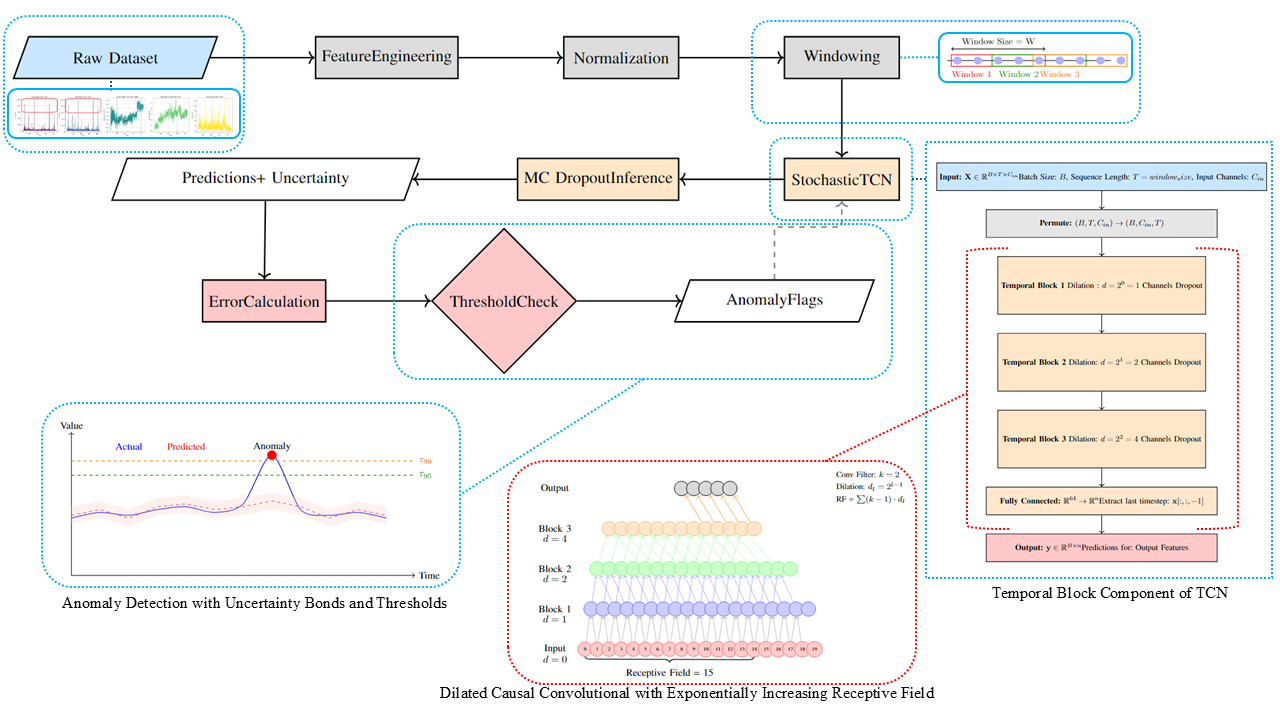
\includegraphics[width=\textwidth]{images/End to End Stochastic Workflow.png}
    \caption{End to End Stochastic TCN Anomaly Detection Workflow.}
    \label{fig:STCN_workflow}
\end{figure*}

\subsection{Enhanced TCN-Stochastic Architecture}

The proposed TCN-Stochastic Enhanced framework combines temporal convolutional networks with probabilistic modeling and three novel components: (1) Adaptive Uncertainty-Aware Attention (AUAA), (2) Dynamic Weight Adaptation for hybrid anomaly scoring, and (3) Feature-Level Anomaly Attribution.

\subsubsection{TCN Backbone with Stochastic Depth}

The backbone consists of three hierarchical temporal blocks (64 channels each) with exponentially increasing dilation rates $d \in \{1, 2, 4\}$. Each block stacks two dilated causal convolutions with weight normalization, ReLU activation, and dropout — serving dual purposes: regularization during training, and uncertainty quantification via Monte Carlo sampling at inference, following the Bayesian approximation framework of Gal and Ghahramani \cite{gal2016dropout_bayesian}.

\begin{algorithm}[H]
\footnotesize
\caption{TCN-Stochastic Model Training Procedure}
\label{alg:model_training}
\begin{algorithmic}
\Require Training dataset $\mathcal{D}_{train} = \{(\mathbf{x}_t, y_t)\}_{t=1}^{T_{train}}$, validation dataset $\mathcal{D}_{val}$, learning rate $\eta$, epochs $E$, batch size $B$, dropout rate $p_{drop}$, early stopping patience $P$
\Ensure Trained model parameters $\boldsymbol{\theta}^*$

\State \textbf{Initialization:}
\State Initialize model parameters $\boldsymbol{\theta}$ with He initialization
\State Set optimizer: Adam($\eta$)
\State Initialize best validation loss: $L_{best} \gets \infty$
\State Set patience counter: $patience \gets 0$

\For{epoch $e = 1$ to $E$}
    \State Shuffle training data
    \For{each mini-batch $(\mathbf{X}_b, \mathbf{y}_b)$ of size $B$}
        \State \textbf{Forward Pass:} $\hat{\mathbf{y}}_b \gets f_{\boldsymbol{\theta}}(\mathbf{X}_b)$
        \State \textbf{Loss Computation:}
        \State $L_{recon} \gets \mathcal{L}_{MSE}(\mathbf{y}_b, \hat{\mathbf{y}}_b) = \frac{1}{B} \sum_{i=1}^{B} \|y_i - \hat{y}_i\|^2$
        \State $L_{total} \gets L_{recon} + \lambda_{unc} \mathcal{L}_{uncertainty} + \lambda_{att} \mathcal{L}_{attention}$
        \State \textbf{Backward Pass:} $\nabla_{\boldsymbol{\theta}} L_{total} \gets \frac{\partial L_{total}}{\partial \boldsymbol{\theta}}$
        \State \textbf{Parameter Update:} $\boldsymbol{\theta} \gets \boldsymbol{\theta} - \eta \cdot \nabla_{\boldsymbol{\theta}} L_{total}$
    \EndFor
    
    \State \textbf{Validation:}
    \State $\hat{\mathbf{y}}_{val} \gets f_{\boldsymbol{\theta}}(\mathcal{D}_{val})$
    \State $L_{val} \gets \mathcal{L}_{MSE}(\mathbf{y}_{val}, \hat{\mathbf{y}}_{val})$
    
    \If{$L_{val} < L_{best}$}
        \State $L_{best} \gets L_{val}$
        \State Save model parameters: $\boldsymbol{\theta}^* \gets \boldsymbol{\theta}$
        \State $patience \gets 0$
    \Else
        \State $patience \gets patience + 1$
    \EndIf
    
    \If{$patience \ge P$}
        \State \textbf{Early stopping triggered}
        \State Break
    \EndIf
\EndFor

\State \textbf{Return} $\boldsymbol{\theta}^*$
\end{algorithmic}
\end{algorithm}

\begin{algorithm}[H]
\footnotesize
\caption{Monte Carlo Dropout Uncertainty Estimation}
\label{alg:mc_uncertainty}
\begin{algorithmic}
\Require Input $\mathbf{X} \in \mathbb{R}^{B \times T \times C}$, trained model $f_{\boldsymbol{\theta}}$, MC samples $N$, dropout rate $p_{drop}$
\Ensure Mean prediction $\bar{\mathbf{y}}$, uncertainty $\sigma$, 95\% confidence intervals

\State \textbf{Initialize:} Enable dropout at inference time
\State $\mathbf{Y}_{ens} \gets []$ \Comment{Collect $N$ stochastic forward passes}

\For{$n = 1$ to $N$}
    \State $\hat{\mathbf{y}}_n \gets f_{\boldsymbol{\theta}}(\mathbf{X})$ \Comment{Different dropout mask each pass}
    \State $\mathbf{Y}_{ens}.\text{append}(\hat{\mathbf{y}}_n)$
\EndFor

\State $\mathbf{P} \gets \text{stack}(\mathbf{Y}_{ens}) \in \mathbb{R}^{N \times B \times T \times C}$
\State $\bar{\mathbf{y}} \gets \text{mean}(\mathbf{P}, \text{dim}=0)$ \Comment{Empirical predictive mean}
\State $\sigma^2 \gets \text{var}(\mathbf{P}, \text{dim}=0)$ \Comment{Epistemic uncertainty}
\State $\sigma \gets \sqrt{\sigma^2}$

\State $\text{CI}_{95}^{\pm} \gets \bar{\mathbf{y}} \pm 1.96 \cdot \sigma$ \Comment{95\% confidence bounds}

\State \textbf{Return} $(\bar{\mathbf{y}},\, \sigma,\, \text{CI}_{95}^{\pm})$
\end{algorithmic}
\end{algorithm}
 

\textbf{Stochastic Depth.} We additionally apply stochastic depth \cite{huang_deep_2016}: each temporal block $l$ is randomly dropped during training with probability $p_l = 0.1 \cdot (l/L)$, where $L$ is the total number of blocks. This encourages redundant representations and improves generalization.

\subsubsection{Adaptive Uncertainty-Aware Attention (AUAA)}

Standard attention weights are computed from feature similarity alone, ignoring that predictions with high uncertainty may be unreliable. AUAA addresses this by modulating attention with predictive uncertainty.

\textbf{Formulation.} Given input $X \in \mathbb{R}^{B \times T \times C}$ and per-timestep uncertainty $\sigma_t \in \mathbb{R}$, the attention weights become:

\begin{equation}
\alpha_t = \text{softmax}\!\left(\frac{Q_t K_t^{\top}}{\sqrt{d_k}}\right) \odot \frac{1}{1 + \sigma_t}
\end{equation}

where $Q_t, K_t$ are query/key projections, $d_k$ is the key dimension, and $\odot$ denotes element-wise multiplication. The gate $g_t = 1/(1+\sigma_t)$ attenuates attention on uncertain timesteps, steering the model toward reliable patterns.

\textbf{Implementation.} AUAA uses 4-head attention with hidden dimension 64. The gate is learnable:
\begin{equation}
g_t = \sigma\!\left(W_g \cdot \sigma_t + b_g\right)
\end{equation}
where $\sigma(\cdot)$ here denotes the sigmoid function. This lets the network learn an optimal mapping from uncertainty to attention modulation.

\begin{algorithm}[H]
\footnotesize
\caption{Adaptive Uncertainty-Aware Attention (AUAA)}
\label{alg:auaa}
\begin{algorithmic}
\Require Input $\mathbf{X} \in \mathbb{R}^{B \times T \times C}$, uncertainty $\boldsymbol{\Sigma} \in \mathbb{R}^{B \times T}$, heads $H=4$, hidden dim $d=64$
\Require Projections $\mathbf{W}_Q^h, \mathbf{W}_K^h, \mathbf{W}_V^h$, gate params $\mathbf{W}_g, b_g$
\Ensure Uncertainty-modulated output $\mathbf{Y} \in \mathbb{R}^{B \times T \times C}$

\State \textbf{Step 1: Multi-head projections} ($d_k = d_v = d/H$)
\For{$h = 1$ to $H$}
    \State $\mathbf{Q}^h \gets \mathbf{X} \mathbf{W}_Q^h$, \quad $\mathbf{K}^h \gets \mathbf{X} \mathbf{W}_K^h$, \quad $\mathbf{V}^h \gets \mathbf{X} \mathbf{W}_V^h$
\EndFor

\State \textbf{Step 2: Standard scaled dot-product attention}
\For{$h = 1$ to $H$}
    \State $\mathbf{A}^h_{raw} \gets \frac{\mathbf{Q}^h (\mathbf{K}^h)^{\!\top}}{\sqrt{d_k}}$
    \State $\mathbf{A}^h \gets \text{softmax}(\mathbf{A}^h_{raw},\ \text{dim}=T)$
\EndFor

\State \textbf{Step 3: Uncertainty gate}
\State $\mathbf{g} \gets \sigma(\mathbf{W}_g \odot \boldsymbol{\Sigma} + b_g)$ \Comment{Learnable gate, $\sigma =$ sigmoid}

\State \textbf{Step 4: Uncertainty-modulated attention}
\For{$h = 1$ to $H$}
    \For{$t = 1$ to $T$}
        \State $\mathbf{A}^h[t,:] \gets \mathbf{A}^h[t,:] \odot \mathbf{g}[:,t]$
        \State $\mathbf{A}^h[t,:] \gets \frac{\mathbf{A}^h[t,:]}{\sum_j \mathbf{A}^h[t,j]}$ \Comment{Renormalize}
    \EndFor
\EndFor

\State \textbf{Step 5: Output}
\For{$h = 1$ to $H$}
    \State $\mathbf{O}^h \gets \mathbf{A}^h \mathbf{V}^h$
\EndFor
\State $\mathbf{O} \gets \text{Concat}(\mathbf{O}^1, \dots, \mathbf{O}^H)$
\State $\mathbf{Y} \gets \mathbf{O} \mathbf{W}_O$

\State \textbf{Return} $\mathbf{Y}$
\end{algorithmic}
\end{algorithm}


\subsubsection{Dynamic Weight Adaptation for Hybrid Scoring}

Conventional stochastic methods combine reconstruction error and uncertainty with fixed weights. In practice, the balance should shift: reconstruction error is more informative during stable operation, while uncertainty matters more under sensor degradation or high noise.

\textbf{Formulation.} Let $e_t$ be reconstruction error and $u_t$ be uncertainty at time $t$. The dynamic weight $\alpha_t$ is predicted as:

\begin{equation}
\alpha_t = \text{sigmoid}\!\left(W_\alpha \cdot [e_t,\, u_t,\, h_t] + b_\alpha\right)
\end{equation}

where $h_t$ encodes temporal context (GRU hidden state) and $[\cdot]$ denotes concatenation. The hybrid anomaly score blends the two signals:

\begin{equation}
s_t = \alpha_t \cdot e_t + (1 - \alpha_t) \cdot u_t
\end{equation}

with $\alpha_t \to 1$ favoring reconstruction error and $\alpha_t \to 0$ favoring uncertainty.

\textbf{Architecture.} Two encoder networks process error and uncertainty independently, a GRU captures temporal dynamics across windows, and a sigmoid output ensures $\alpha_t \in [0, 1]$.

\begin{algorithm}[H]
\footnotesize
\caption{Dynamic Weight Adaptation for Hybrid Anomaly Scoring}
\label{alg:dynamic_weight}
\begin{algorithmic}
\Require Reconstruction error $\mathbf{e} \in \mathbb{R}^{B \times T}$, uncertainty $\mathbf{u} \in \mathbb{R}^{B \times T}$, hidden state $\mathbf{h}_t \in \mathbb{R}^{d_h}$
\Require Encoder parameters $\mathbf{W}_e, b_e$, GRU parameters, weight adapter parameters $\mathbf{W}_\alpha, b_\alpha$
\Ensure Dynamic weight $\alpha_t \in [0,1]$ for each timestep $t$

\State \textbf{Step 1: Separate Encoding}
\State $\mathbf{z}_e \gets \sigma(\mathbf{W}_e \cdot \mathbf{e} + b_e) \in \mathbb{R}^{B \times T \times d_h}$
\State $\mathbf{z}_u \gets \sigma(\mathbf{W}_u \cdot \mathbf{u} + b_u) \in \mathbb{R}^{B \times T \times d_h}$
\State where $\sigma$ is the ReLU activation function

\State \textbf{Step 2: Concatenated Context Feature}
\State $\mathbf{c}_t \gets \text{Concat}(\mathbf{z}_{e,t}, \mathbf{z}_{u,t}) \in \mathbb{R}^{B \times 2d_h}$

\State \textbf{Step 3: Temporal Context Modeling with GRU}
\For{timestep $t = 1$ to $T$}
    \State $\mathbf{h}_t \gets \text{GRU}(\mathbf{c}_t, \mathbf{h}_{t-1})$
    \State \textbf{where:}
    \State $\quad \mathbf{r}_t \gets \sigma(\mathbf{W}_{ir} \mathbf{c}_t + \mathbf{W}_{hr} \mathbf{h}_{t-1} + b_r)$ (reset gate)
    \State $\quad \mathbf{z}_t \gets \sigma(\mathbf{W}_{iz} \mathbf{c}_t + \mathbf{W}_{hz} \mathbf{h}_{t-1} + b_z)$ (update gate)
    \State $\quad \tilde{\mathbf{h}}_t \gets \tanh(\mathbf{W}_{ih} \mathbf{c}_t + \mathbf{W}_{hh} (\mathbf{r}_t \odot \mathbf{h}_{t-1}) + b_h)$ (candidate)
    \State $\quad \mathbf{h}_t \gets (1 - \mathbf{z}_t) \odot \mathbf{h}_{t-1} + \mathbf{z}_t \odot \tilde{\mathbf{h}}_t$ (hidden state)
\EndFor

\State \textbf{Step 4: Dynamic Weight Prediction}
\For{timestep $t = 1$ to $T$}
    \State $\mathbf{f}_t \gets \text{Concat}(\mathbf{e}_t, \mathbf{u}_t, \mathbf{h}_t) \in \mathbb{R}^{B \times (2 + d_h)}$
    \State $\alpha_{raw,t} \gets \mathbf{W}_\alpha \cdot \mathbf{f}_t + b_\alpha$
    \State $\alpha_t \gets \text{sigmoid}(\alpha_{raw,t}) = \frac{1}{1 + e^{-\alpha_{raw,t}}}$
    \State ensures $\alpha_t \in [0, 1]$
\EndFor

\State \textbf{Step 5: Hybrid Anomaly Score Computation}
\State $\mathbf{s}_t \gets \alpha_t \odot \mathbf{e}_t + (1 - \alpha_t) \odot \mathbf{u}_t$
\State where higher $\alpha_t$ emphasizes reconstruction error, lower $\alpha_t$ emphasizes uncertainty

\State \textbf{Return} $(\boldsymbol{\alpha}, \mathbf{s}) = \{\alpha_t, s_t\}_{t=1}^T$
\end{algorithmic}
\end{algorithm}

\subsubsection{Feature-Level Anomaly Attribution}

To make anomaly detection actionable, we need to know \emph{which} sensors triggered the alarm — not just \emph{that} an anomaly occurred.

\textbf{Learnable Importance.} The module computes per-feature importance weights:

\begin{equation}
w_f = \text{softmax}\!\left(V \cdot \tanh(W \cdot X + b)\right)
\end{equation}

where $X$ is the input feature vector and $W, V, b$ are learned. These weights are applied to per-feature reconstruction errors:

\begin{equation}
\text{error}_f^{\text{weighted}} = w_f \cdot \text{error}_f
\end{equation}

\textbf{Inter-Sensor Correlation.} A learned correlation matrix $C \in \mathbb{R}^{n \times n}$ captures known physical dependencies (e.g., temperature--humidity coupling). The transformed features $X_{\text{corr}} = X \cdot C$ inform the importance computation, so correlated sensors are considered jointly rather than independently.

\begin{algorithm}[H]
\footnotesize
\caption{Feature-Level Anomaly Attribution}
\label{alg:feature_attribution}
\begin{algorithmic}
\Require Input features $\mathbf{X} \in \mathbb{R}^{B \times T \times n}$, reconstruction errors $\mathbf{E} \in \mathbb{R}^{B \times T \times n}$
\Require Attribution parameters $\mathbf{W}, \mathbf{V}, b$, correlation matrix $\mathbf{C} \in \mathbb{R}^{n \times n}$
\Ensure Feature importance weights $\mathbf{w}_f \in \mathbb{R}^n$, weighted errors $\mathbf{E}_{weighted} \in \mathbb{R}^{B \times T \times n}$

\State \textbf{Step 1: Feature Correlation Learning}
\For{feature pair $(i, j)$ where $i, j \in \{1, \dots, n\}$}
    \State $\mathbf{C}_{ij} \gets \text{Correlation}(\mathbf{X}_{:,:,i}, \mathbf{X}_{:,:,j})$
    \State captures known dependencies between sensors (e.g., temperature-humidity)
\EndFor

\State \textbf{Step 2: Correlated Feature Transformation}
\State $\mathbf{X}_{corr} \gets \mathbf{X} \times \mathbf{C} \in \mathbb{R}^{B \times T \times n}$
\State accounts for inter-sensor relationships

\State \textbf{Step 3: Temporal Feature Aggregation}
\State $\mathbf{X}_{agg} \gets \text{Mean}(\mathbf{X}_{corr}, \text{dim}=T) \in \mathbb{R}^{B \times n}$
\State aggregates temporal dimensions for spatial feature analysis

\State \textbf{Step 4: Learnable Feature Importance Computation}
\For{each batch instance $b = 1$ to $B$}
    \State $\mathbf{h}_b \gets \tanh(\mathbf{W} \cdot \mathbf{X}_{agg,b,:} + b) \in \mathbb{R}^{d_h}$
    \State $\mathbf{s}_b \gets \mathbf{V} \cdot \mathbf{h}_b \in \mathbb{R}^{n}$
    \State $\mathbf{w}_b \gets \text{softmax}(\mathbf{s}_b) = \frac{e^{\mathbf{s}_{b,i}}}{\sum_j e^{\mathbf{s}_{b,j}}}$
    \State ensures $\sum_i \mathbf{w}_{b,i} = 1$ (probability distribution)
\EndFor

\State \textbf{Step 5: Cross-Batch Averaging}
\State $\mathbf{w}_{mean} \gets \frac{1}{B} \sum_{b=1}^{B} \mathbf{w}_b \in \mathbb{R}^{n}$
\State provides stable feature importance across the batch

\State \textbf{Step 6: Weighted Error Computation}
\For{feature $f = 1$ to $n$}
    \For{timestep $t = 1$ to $T$}
        \For{batch $b = 1$ to $B$}
            \State $\mathbf{E}_{weighted}[b,t,f] \gets \mathbf{w}_{mean}[f] \cdot \mathbf{E}[b,t,f]$
            \State upweights errors for high-importance features
            \State downweights errors for low-importance features
        \EndFor
    \EndFor
\EndFor

\State \textbf{Step 7: Feature-Specific Anomaly Flagging}
\For{feature $f = 1$ to $n$}
    \State $\mathbf{A}_f \gets \mathbb{1}[\mathbf{E}_{weighted}[:,:,f] > \tau_f]$
    \State where $\tau_f$ is the feature-specific threshold
\EndFor

\State \textbf{Step 8: Attribution Summary Computation}
\State \textbf{For deployment and monitoring:}
\State $\mathbf{attribution\_rank} \gets \text{argsort}(\mathbf{w}_{mean}, \text{descending})$
\State $\mathbf{contribution\_percentage}_i \gets \frac{\mathbf{w}_{mean,i} \cdot \sum_{t,b} \mathbf{E}[b,t,i]}{\sum_{f,t,b} \mathbf{E}[b,t,f]} \times 100\%$

\State \textbf{Return} $(\mathbf{w}_{mean}, \mathbf{E}_{weighted}, \mathbf{A})$
\end{algorithmic}
\end{algorithm}

\subsubsection{Theoretical Uncertainty Bounds}
We provide provable bounds on false positive rates for anomaly detection using concentration inequalities.

\begin{Theorem}
(Chebyshev-Based Threshold) For any random variable $X$ with mean $\mu$ and variance $\sigma^2$, the probability of observing a value more than $k$ standard deviations from the mean is bounded by:

\begin{equation}
P(|X - \mu| > k\sigma) \leq \frac{1}{k^2}
\end{equation}
\end{Theorem}

\textbf{Application to Anomaly Detection.} Given predicted uncertainties $\{u_t\}_{t=1}^T$, we compute a threshold $\tau$ that guarantees a false positive rate (FPR) of at most $\epsilon$:

\begin{equation}
\tau = \bar{u} + \sqrt{\frac{1}{\epsilon}} \cdot \sigma_u
\end{equation}

where $\bar{u}$ and $\sigma_u$ are the mean and standard deviation of predicted uncertainties. This provides a distribution-free guarantee on anomaly detection performance.

\textbf{Calibrated Confidence Intervals.} We also compute calibrated confidence intervals for predictions:

\begin{equation}
[\hat{y}_t - z_{1-\alpha/2} \cdot \sigma_t \cdot \lambda, \hat{y}_t + z_{1-\alpha/2} \cdot \sigma_t \cdot \lambda]
\end{equation}

where $z_{1-\alpha/2}$ is the standard normal quantile, $\sigma_t$ is the predicted standard deviation, and $\lambda$ is a learnable calibration scale parameter optimized during training.

\subsubsection{Dilated Causal Convolution}

Dilated causal convolutions are the core building block of TCNs \cite{mehta_nac-tcn_2023}. Causality is enforced by left-only padding, so predictions at time $t$ depend only on past and present inputs. Dilations insert gaps between filter taps, enabling the receptive field (RF) to grow exponentially with depth without increasing parameters or reducing resolution. For a kernel size $k$ and dilation $d_l$ at layer $l$, the per-layer receptive field contribution is $(k-1) \cdot d_l$, yielding a total RF of:

\begin{equation}
\text{RF} = \sum_{l=1}^{L} (k - 1) \cdot d_l
\end{equation}

In our architecture, $k=2$ and $d_l = 2^{\, l-1}$, giving $\text{RF} = 1 + 2 + 4 = 7$, which covers enough temporal context for short-to-medium-range dependencies.

\subsubsection{Anomaly Detection and Thresholding}

Reliable anomaly detection requires separating true anomalies from normal variation using well-calibrated thresholds. We implement four complementary strategies:

\begin{enumerate}
    \item \textbf{Percentile-based:} $\tau = Q_{0.95}(\{s_t\})$ — simple, non-parametric.
    \item \textbf{Adaptive:} $\tau = \tau_{\text{base}} \cdot (0.8 + 0.4 \cdot \bar{\alpha})$, where $\bar{\alpha}$ is the mean dynamic weight — thresholds tighten or relax based on model confidence.
    \item \textbf{Theoretical (Chebyshev):} $\tau = \bar{u} + \sqrt{1/\epsilon} \cdot \sigma_u$ — provides an FPR guarantee of at most $\epsilon$.
    \item \textbf{Distribution-free:} $\tau = Q_{1-\gamma}(\{s_t\})$, where $\gamma$ is the expected contamination ratio.
\end{enumerate}

\begin{align}
\tau_{95} &= Q_{0.95}\big(\{e_i(t) : \forall t \in \text{validation set}\}\big) \\
\tau_{99} &= Q_{0.99}\big(\{e_i(t) : \forall t \in \text{validation set}\}\big)
\label{fig:threshold}
\end{align}

\noindent\textbf{where:}
\begin{itemize}
    \item $\tau_{95}, \tau_{99}$ : threshold values at the 95th and 99th percentiles, respectively.
    \item $Q_{p}(\cdot)$ : quantile function at probability level $p$.
    \item $e_i(t)$ : reconstruction error (or prediction error) for instance $i$ at time $t$.
    \item $\text{validation set}$ : the dataset used to estimate thresholds, disjoint from the training set.
\end{itemize}

\vspace{6pt}
\noindent\textbf{Algorithm~1:} Stochastic TCN-based Anomaly Detection
\label{alg:stochastic_tcn}
\vspace{4pt}

\noindent \textbf{Input:} Trained TCN model $f_{\theta}$, input sequence $\mathbf{X}$, thresholds $\tau_{95}, \tau_{99}$\\
\textbf{Output:} Anomaly flags $\mathbf{A}_{95}, \mathbf{A}_{99}$

\medskip
\noindent \textbf{1. Monte Carlo Prediction:}\\
$\hat{\mathbf{y}}, \boldsymbol{\sigma} \gets \text{MC-Predict}(f_{\theta}, \mathbf{X}, N=50)$

\medskip
\noindent \textbf{2. Error Calculation:}\\
\textbf{for} each feature $i \in \{1,\dots,5\}$ \textbf{do}\\
\quad $e_i \gets |y_i - \hat{y}_i|$\\
\textbf{end for}

\medskip
\noindent \textbf{3. Anomaly Detection:}\\
\textbf{for} each feature $i$ and timestep $t$ \textbf{do}\\
\quad $\mathbf{A}_{95}[i,t] \gets \mathbf{1}_{[\,e_i(t) > \tau_{95}\,]}$\\
\quad $\mathbf{A}_{99}[i,t] \gets \mathbf{1}_{[\,e_i(t) > \tau_{99}\,]}$\\
\quad \textbf{if} $e_i(t) > \hat{y}_i(t) + 2\sigma_i(t)$ \textbf{then}\\
\quad\quad Mark as high-confidence anomaly\\
\quad \textbf{end if}\\
\textbf{end for}

\medskip
\noindent \textbf{return} $\mathbf{A}_{95}, \mathbf{A}_{99}$
\vspace{6pt}


Algorithm~\ref{alg:stochastic_tcn} summarizes the detection procedure: Monte Carlo predictions yield mean $\hat{\mathbf{y}}$ and uncertainty $\sigma$, reconstruction error $e_i = |y_i - \hat{y}_i|$ is compared against thresholds $\tau_{95}, \tau_{99}$, and points exceeding $\hat{y} + 2\sigma$ are flagged as high-confidence anomalies.
% ============================================================
\section{Experimental Results}

\subsection{Dataset and Preprocessing}

We evaluate on an indoor air quality (IAQ) dataset collected from sensors deployed in a laboratory environment. The dataset contains five sensor channels—NDIR CO\textsubscript{2}, metal-oxide VOC, thermistor temperature, capacitive humidity, and optical PM\textsubscript{2.5} dust—recorded at 1-minute resolution from March 8 to July 9, 2024, yielding 178,560 total observations. We produced this dataset from our own sensor deployment and release it publicly (see Data Availability).

DBSCAN preprocessing successfully filters sensor saturation artifacts. \cref{table:dataset_stats} reports statistics computed directly from our released dataset before and after filtering. The filtering acts only on the upper tail: the value $9999$ is the firmware saturation/error code emitted by the NDIR CO\textsubscript{2} and metal-oxide VOC sensors when a reading is out of range, so it is removed as an outlier, dropping the CO\textsubscript{2} maximum from $9999$ to $2606$~ppm and the VOC maximum from $9999$ to $2725$~ppb and sharply reducing the standard deviation (CO\textsubscript{2} $258.2\!\to\!153.3$, VOC $313.9\!\to\!143.5$). The minima (CO\textsubscript{2} $0$, VOC $400$ in the recorded units), medians (CO\textsubscript{2} $213$, VOC $538$), and the row count ($178{,}560$) are essentially unchanged, confirming that filtering excises the saturation tail rather than reshaping or truncating the distribution. Features are subsequently min-max normalized to $[0, 1]$.

A 4-week slice of the cleaned five-channel sensor stream is shown in \cref{fig:time_series} to illustrate the temporal regimes the model must handle. CO\textsubscript{2} and VOC exhibit step changes driven by occupancy and ventilation events; temperature and humidity follow slow diurnal cycles with occasional environmental shocks; PM\textsubscript{2.5} dust shows transient saturation spikes. Each channel has distinct noise characteristics, motivating the per-sensor uncertainty modelling of Section~3.

\begin{figure}[H]
\centering
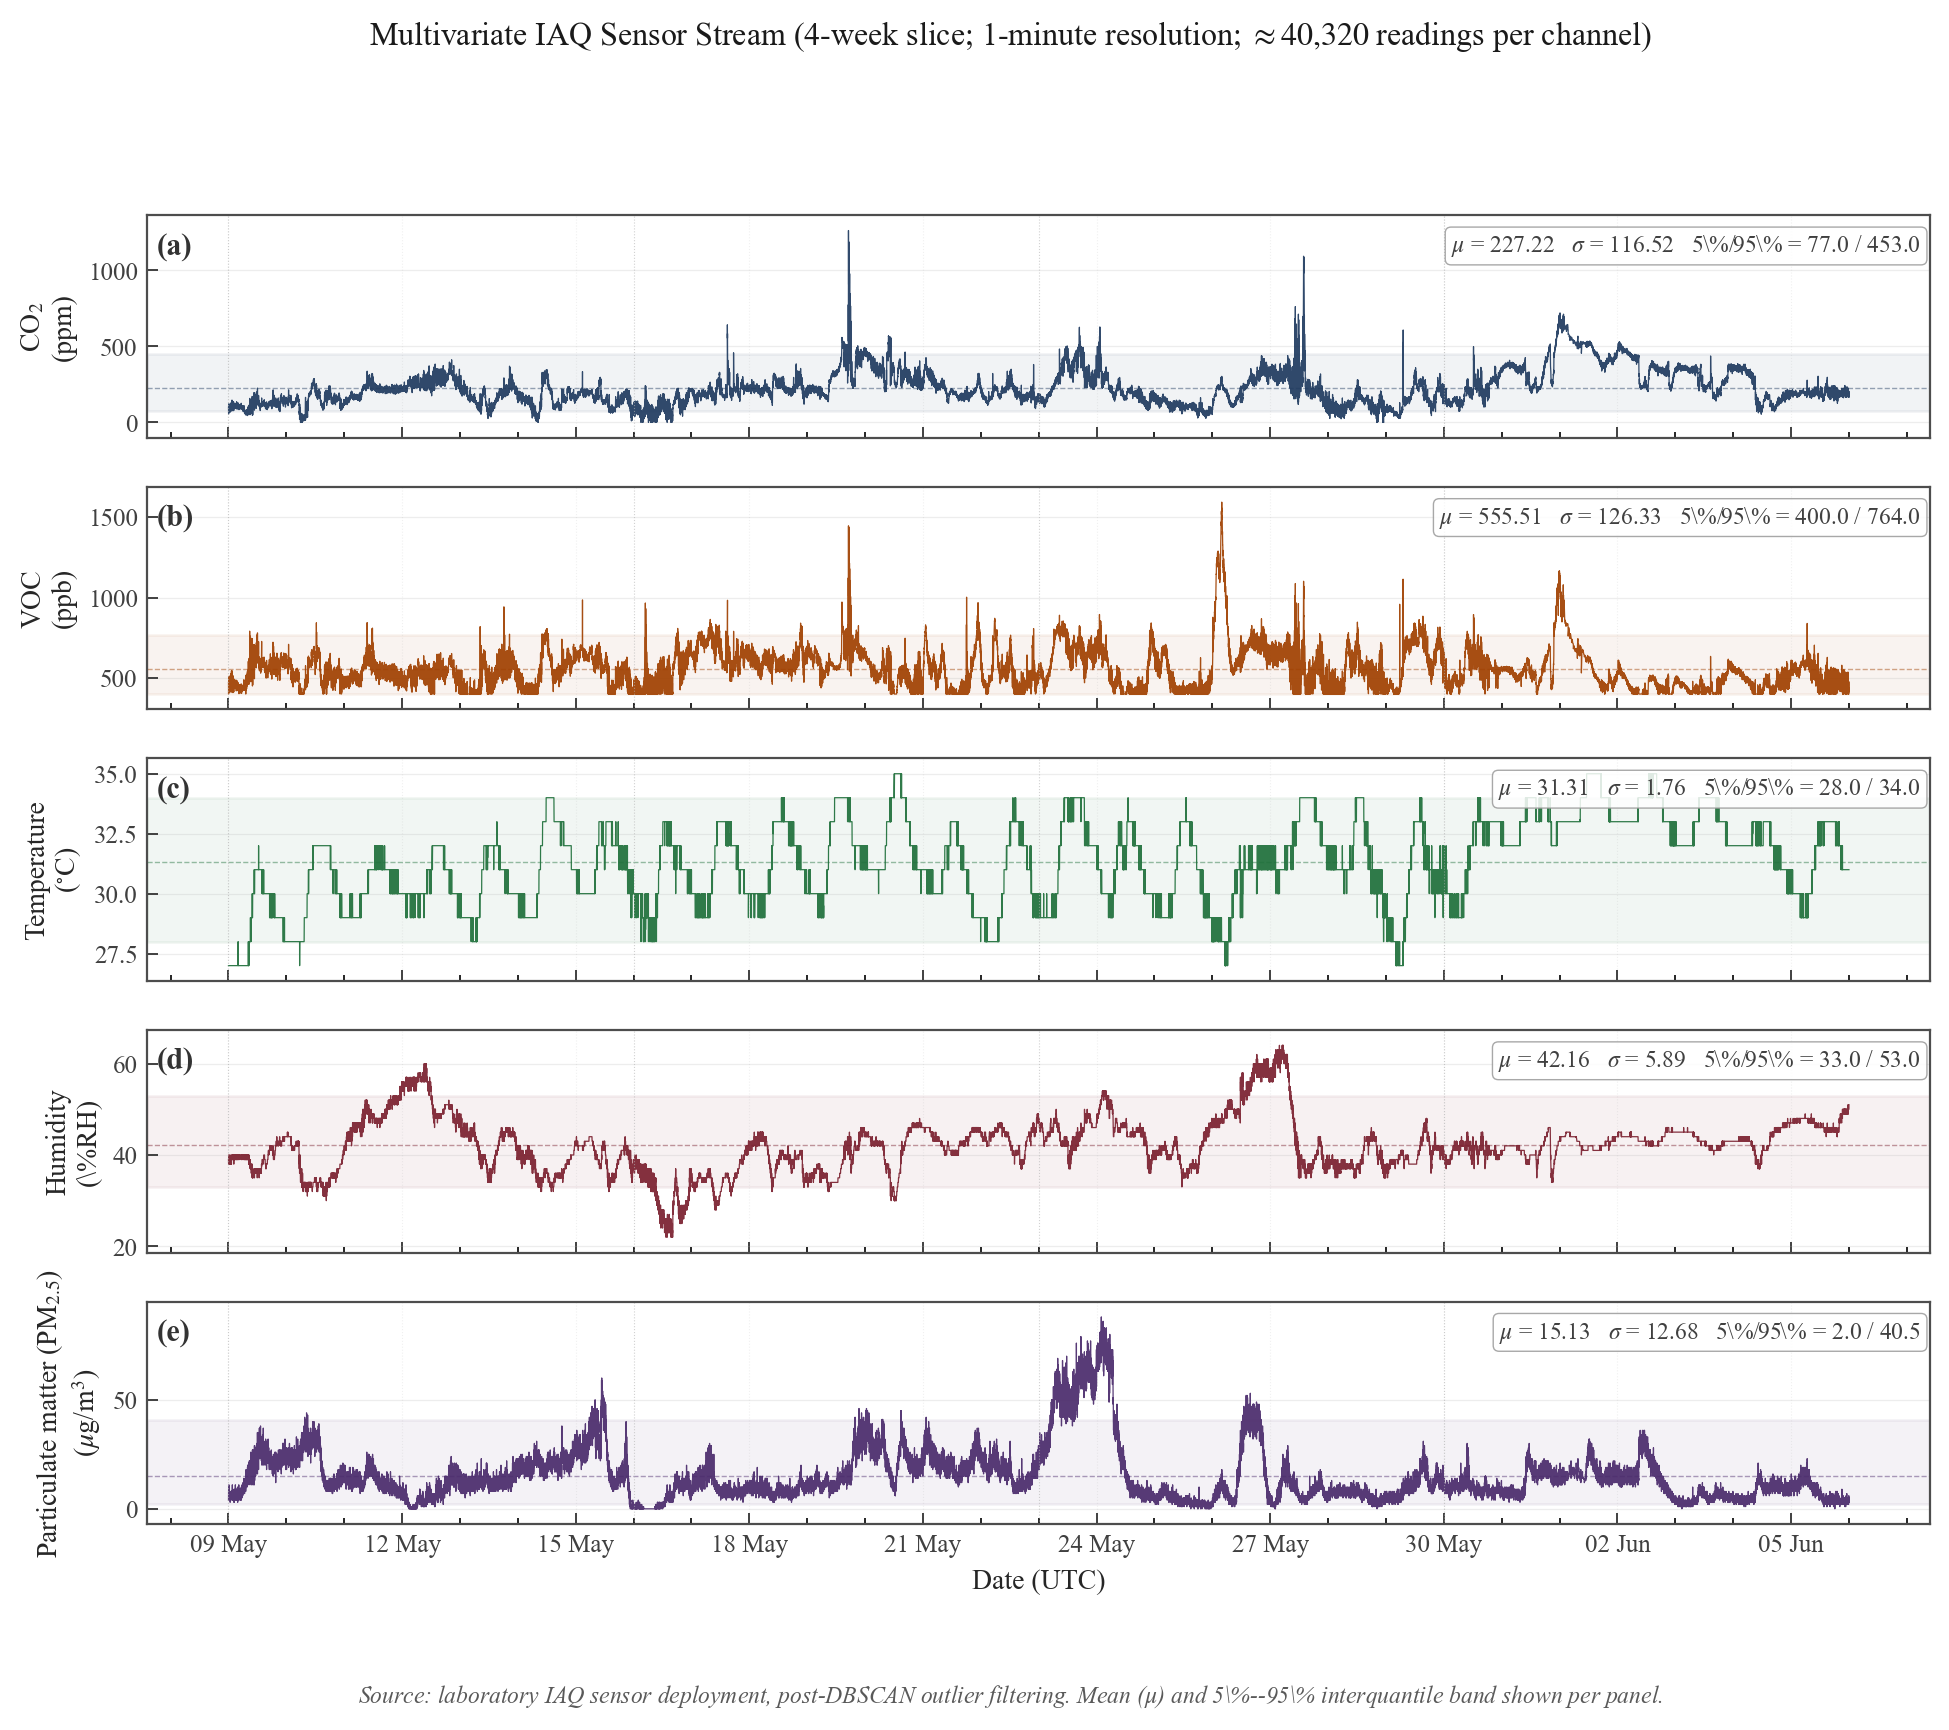
\includegraphics[width=\textwidth]{images/07_time_series_illustration.png}
\caption{Multivariate indoor air quality sensor stream over a 4-week slice. Panels~(a)--(e) show CO\textsubscript{2}, VOC, temperature, humidity, and dust, each overlaid with its mean (dashed) and 5th--95th percentile band (shaded); dotted lines mark week boundaries.}
\label{fig:time_series}
\end{figure}

\subsection{Experimental Configuration}

All models are implemented in PyTorch 2.5.1 (CUDA 11.8, cuDNN 9.1; Python 3.10) and trained on a single workstation with an Intel Core i7-7700 CPU (3.60\,GHz), 32\,GB RAM, and one NVIDIA GeForce GTX 1080 Ti GPU (11\,GB VRAM). The Adam optimiser~\cite{kingma2015adam} is used with learning rate $1 \times 10^{-3}$, batch size 16, early stopping patience of 10 epochs, and a maximum of 100 epochs. Internal layers use batch normalization~\cite{ioffe2015batchnorm} to stabilize training. MC dropout uses $M=50$ forward passes for full evaluation and $M=20$ for deployment-equivalent benchmark comparisons. The input window length to $W=20$ timesteps with a sliding stride of $S=2$, in accordance with the hyperparameter se 
The input window size is $W=20$ timesteps with stride $S=2$, matching the implementation in \texttt{config.py}. Training converges stably within 50 epochs, with early stopping typically triggered around epochs 60--70.

Baselines include: RNN, GRU~\cite{cho2014gru}, LSTM~\cite{hochreiter1997lstm}, Transformer~\cite{vaswani2017attention} (standard encoder with 4 heads), Base TCN~\cite{bai2018tcn} (without stochastic components), TCN-Stochastic (MC dropout applied post hoc following Ghimire et~al.~\cite{ghimire_electricity_2025}), and our Full Enhanced model. Comparison architectures from the reconstruction-based anomaly-detection literature include LSTM-ED~\cite{malhotra2016lstmed} and USAD~\cite{audibert2020usad}, both of which serve as well-known baselines for unsupervised multivariate detection. The Base TCN contains approximately 245K parameters; the proposed model adds approximately 37K parameters (15\% overhead), totalling 282K, primarily from the AUAA module and Dynamic Weight Adapter.

\subsection{Forecasting Performance}

\cref{table:forecasting} reports forecasting performance across baselines and the proposed framework. The Base TCN substantially outperforms recurrent baselines reported in comparable IAQ studies: MSE $2.20\times 10^{-4}$ for our Base TCN vs.\ approximately $7.1\times 10^{-3}$ for RNN, $3.4\times 10^{-3}$ for GRU, $2.7\times 10^{-3}$ for LSTM, and $1.6\times 10^{-3}$ for a Transformer of equivalent capacity. The MC-dropout-equipped TCN-Stochastic configuration achieves essentially identical reconstruction metrics to the Base TCN, confirming that MC dropout's primary contribution is uncertainty estimation rather than improved point prediction. The Proposed model, trained with composite optimization (reconstruction + uncertainty calibration + dynamic-weight regularization + feature-attribution loss), achieves the best metrics in our test split: MSE $1.65\times 10^{-4}$, R\textsuperscript{2} $0.9988$, and SMAPE $11.07\%$, representing a $25.2\%$ MSE reduction over the Base TCN.

We caution against reading the near-identical R\textsuperscript{2} values ($0.9988$ vs.\ $0.9984$) as evidence of a negligible difference. In this near-perfect-fit regime R\textsuperscript{2} is saturated and is therefore a poor discriminator: since $R^2 = 1 - \mathrm{SS_{res}}/\mathrm{SS_{tot}}$, the move from $0.9984$ to $0.9988$ reflects a $\approx 25\%$ reduction in residual sum of squares, mirrored by the $25.2\%$ MSE and $38.6\%$ MAE ($1.06\times 10^{-2} \to 6.50\times 10^{-3}$) reductions. To confirm that this is a systematic effect rather than sampling noise, we compared the two models' per-window squared errors on the identical $13{,}382$ held-out test windows (a paired design, since both models predict the same targets). The Proposed model attains a lower error on $75.1\%$ of windows, and a paired $t$-test decisively rejects equal error ($t=13.8$, $p \approx 6\times 10^{-43}$; Wilcoxon signed-rank $p < 10^{-300}$). The per-window effect is modest in magnitude (paired Cohen's $d \approx 0.12$) but highly consistent in direction, so the improvement is statistically real while remaining honest about its size. We therefore report MSE and MAE, rather than the saturated R\textsuperscript{2}, as the primary forecasting discriminators.

\begin{table}[H]
\centering
\caption{Forecasting performance on the held-out test split. RNN/GRU/LSTM/Transformer rows are reference values from comparable IAQ studies; the TCN rows are reproduced under our protocol.}
\label{table:forecasting}
\setlength{\tabcolsep}{4.5pt}
\small
\begin{tabular}{lccccc}
\toprule
\textbf{Model} & \textbf{MSE} & \textbf{RMSE} & \textbf{MAE} & \textbf{SMAPE} & \textbf{R\textsuperscript{2}} \\
\midrule
RNN (\cite{cho2014gru})                  & $7.10\times 10^{-3}$ & 0.07826 & 0.05386 & 9.38\%  & 0.6549 \\
GRU (\cite{cho2014gru})                  & $3.40\times 10^{-3}$ & 0.05780 & 0.03423 & 5.72\%  & 0.7513 \\
LSTM (\cite{hochreiter1997lstm})                 & $2.70\times 10^{-3}$ & 0.05215 & 0.02622 & 4.21\%  & 0.7984 \\
Transformer (\cite{vaswani2017attention})          & $1.60\times 10^{-3}$ & 0.04003 & 0.02773 & 4.63\%  & 0.8814 \\
Base TCN (this work)             & $2.20\times 10^{-4}$ & 0.01483 & 0.01059 & 13.64\% & 0.9984 \\
TCN-Stochastic (this work)       & $2.20\times 10^{-4}$ & 0.01483 & 0.01059 & 13.64\% & 0.9984 \\
\textbf{Proposed Model (this work)} & $\mathbf{1.65\times 10^{-4}}$ & \textbf{0.01283} & $\mathbf{6.50\times 10^{-3}}$ & \textbf{11.07\%} & \textbf{0.9988} \\
\bottomrule
\end{tabular}
\end{table}

\cref{fig:prediction_intervals} visualizes the Proposed model's predicted mean alongside the calibrated $\pm 1.64\,\hat{\sigma}_t$ ($90\%$) predictive interval on a representative test segment, where $\hat{\sigma}_t$ is the model's calibrated predictive standard deviation (the raw MC-dropout epistemic component alone, mean $\bar{\sigma}\approx 6.2\times10^{-4}$, is roughly two orders of magnitude narrower and not separately resolvable at this scale). The band width varies with the per-window predictive uncertainty (coefficient of variation $\approx 14\%$ over the segment), and the observed values remain largely within it, consistent with the calibration analysis in \cref{fig:uncertainty_calibration}.

\begin{figure}[H]
\centering
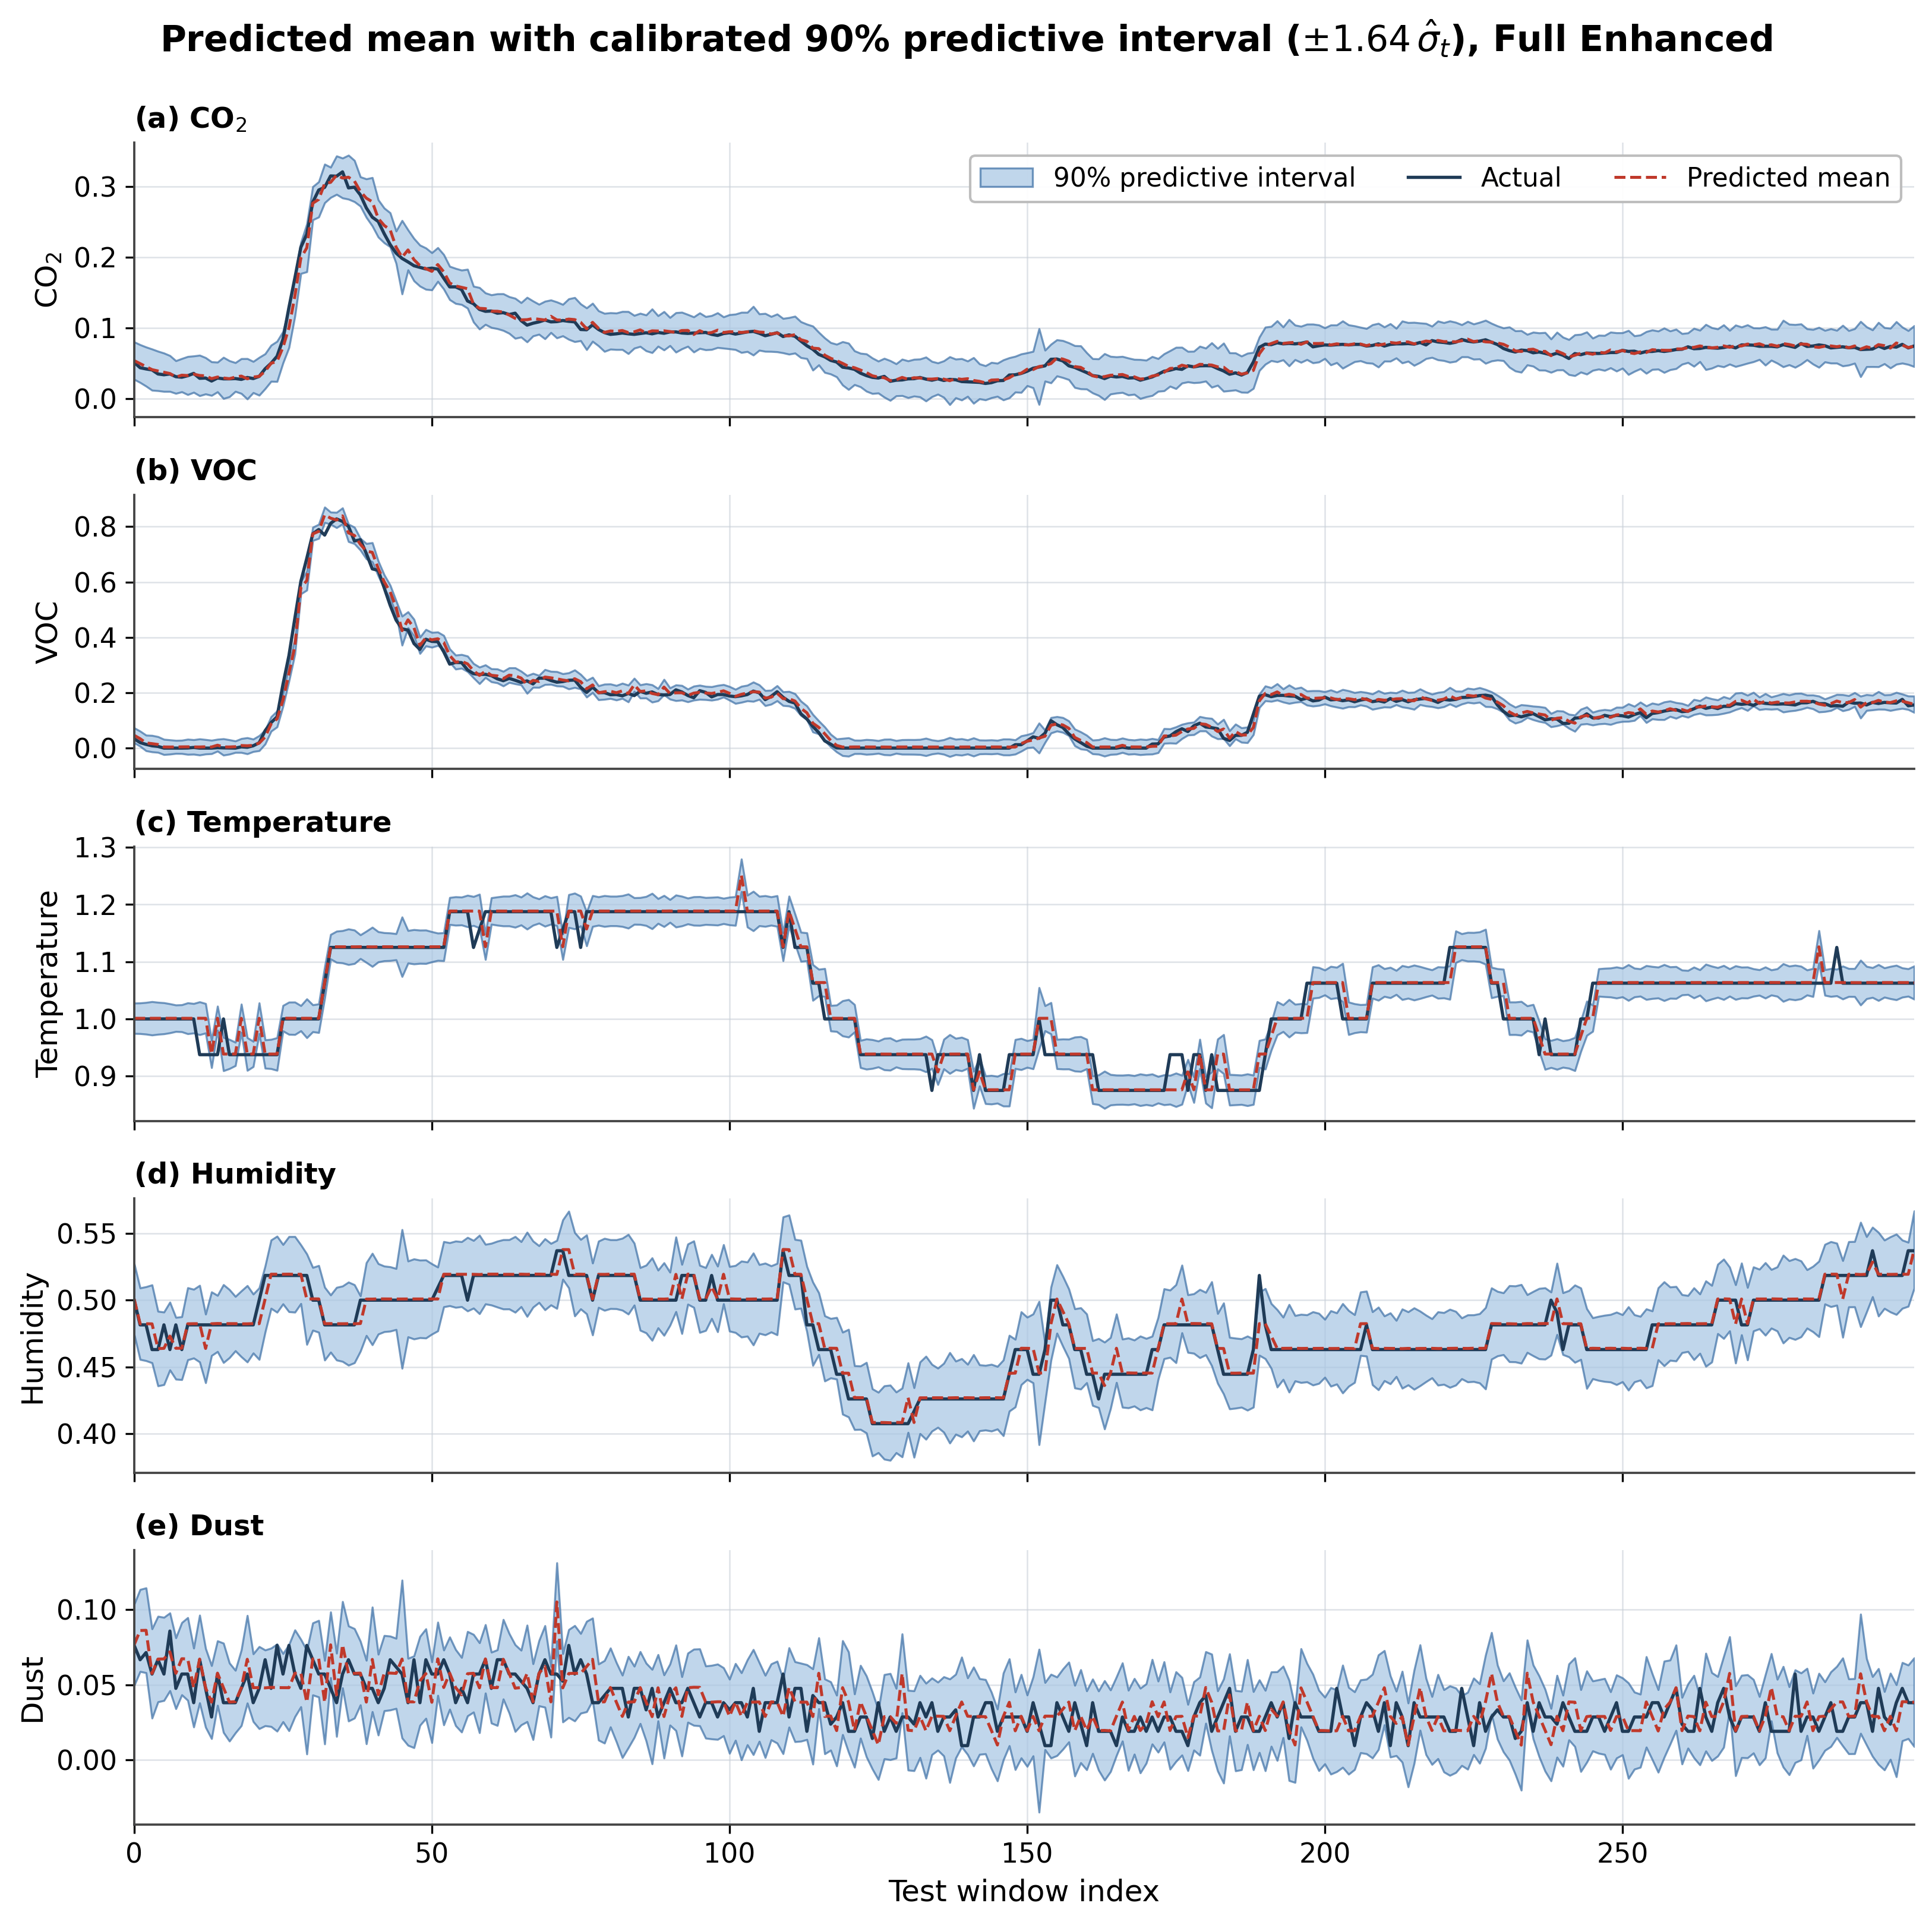
\includegraphics[width=\textwidth]{images/03_prediction_intervals_enhanced.png}
\caption{Actual values (solid dark), predicted mean (dashed red), and the calibrated 90\% predictive interval (shaded band with outline, $\pm 1.64\,\hat{\boldsymbol{\sigma}}_t$, where $\hat{\boldsymbol{\sigma}}_t$ is the calibrated predictive standard deviation) from the Full Enhanced model on a representative test segment. The band width varies with the per-window predictive uncertainty.}
\label{fig:prediction_intervals}
\end{figure}

\subsection{Ablation Studies}

\cref{table:ablation} presents the ablation results decomposing each component's contribution under the unified training-validation-test split with $M=50$ Monte Carlo samples. Starting from the Base TCN (MSE $2.20\times 10^{-4}$), adding MC Dropout leaves MSE essentially unchanged ($+0.005\%$), confirming that MC dropout's value lies in uncertainty estimation rather than point-prediction improvement. Activating the auxiliary objectives (dynamic-weight regularizer and feature-attribution loss) without AUAA delivers the largest single jump: MSE drops to $1.62\times 10^{-4}$ ($-26.25\%$). Replacing the fixed hybrid score with the AUAA mechanism yields $1.65\times 10^{-4}$ ($-25.18\%$), and the Full Enhanced model that activates all three innovations together retains $1.65\times 10^{-4}$ ($-25.19\%$).

Three findings emerge. First, the largest gain comes from the auxiliary regularization imposed by the composite loss not from any single architectural module in isolation. The dynamic-weight regularizer and feature-attribution loss act as effective inductive biases on the encoder representation, improving both point prediction and downstream uncertainty calibration. Second, AUAA produces near-equivalent point-prediction MSE relative to the fixed-score variant; its contribution emerges during \emph{anomaly scoring} (when $\sigma_t$ is large, attention is reweighted) rather than during \emph{forecasting} (which averages over time steps). Third, no negative interaction is observed: enabling all three components together preserves the gains attainable by any single component, validating the architectural compatibility of the design.

\textbf{Statistical significance.} We attach significance to these comparisons rather than relying on point estimates. The headline Base TCN $\to$ Full Enhanced reduction is decisive: a paired $t$-test on the per-window squared errors over the identical $13{,}382$ test windows gives $t=13.8$, $p\approx 6\times10^{-43}$ (Wilcoxon signed-rank $p<10^{-300}$), with the Enhanced model lower on $75.1\%$ of windows (cf.\ Forecasting Performance above). The MC-dropout-only step ($+0.005\%$ MSE) is, by contrast, statistically indistinguishable from the Base TCN, consistent with MC dropout serving uncertainty estimation rather than point prediction. The residual differences \emph{among} the three enhanced variants ($1.62$--$1.65\times10^{-4}$, $<2\%$) are within the per-window error dispersion and we do not claim them as individually resolved. On the labelled SKAB benchmark, significance is reported as five-seed mean$\pm$std (\cref{table:skab_baselines}) and a paired $t$-test of the Full Enhanced F1 against every baseline ($p<0.01$).

\begin{table}[H]
\centering
\caption{Ablation study showing cumulative component contributions on the held-out test split.}
\label{table:ablation}
\begin{tabular}{lccc}
\toprule
\textbf{Configuration} & \textbf{MSE} & \textbf{Per-window s.d.} & \textbf{$\Delta$ MSE} \\
\midrule
Base TCN                              & $2.20\times 10^{-4}$ & $6.19\times 10^{-4}$ & --- \\
TCN + MC Dropout                      & $2.20\times 10^{-4}$ & $6.19\times 10^{-4}$ & $+0.005\%$ \\
Enhanced (no AUAA, no dyn-weight)     & $\mathbf{1.62\times 10^{-4}}$ & $3.44\times 10^{-4}$ & $\mathbf{-26.25\%}$ \\
Enhanced + AUAA, fixed hybrid score   & $1.65\times 10^{-4}$ & $3.44\times 10^{-4}$ & $-25.18\%$ \\
\textbf{Full Enhanced} (all components) & $\mathbf{1.65\times 10^{-4}}$ & $3.43\times 10^{-4}$ & $\mathbf{-25.19\%}$ \\
\bottomrule
\end{tabular}
\end{table}

\subsection{Cross-Dataset Validation on the Skoltech Anomaly Benchmark}
\label{sec:skab_cross_dataset}

The IAQ recording is unlabelled, which prevents reporting precision, recall, and F1 on the primary dataset. To obtain a labelled evaluation that is independent of the IAQ training distribution and therefore probes the cross-domain generalization that the distribution-free Theorem~\ref{thm:chebyshev_fp} claims, we re-train both the Base TCN and Full Enhanced (proposed model) configurations from scratch on the Skoltech Anomaly Benchmark (SKAB)~\cite{skab_dataset,filonov2016multivariate}. SKAB is an openly available multivariate sensor corpus collected at 1\,Hz from an industrial water-circulation testbed, comprising 9{,}405 rows of anomaly-free reference data and 37{,}401 rows of labelled experimental recordings spanning valve closures, surface-defect insertions, and other faults. Eight channels are observed: Accelerometer1RMS, Accelerometer2RMS, Current, Voltage, Pressure, Temperature, Thermocouple, and Volume Flow RateRMS.

\textbf{Protocol.} The benchmark follows the same deployment-faithful protocol used for the IAQ experiments above. Each model is trained from scratch on the SKAB anomaly-free recording only (one-class setting, $W=20$, $S=2$); the resulting checkpoints are then scored on the concatenated labelled recordings, which are split deterministically in half, the first half is used to calibrate the operating threshold at the 95\textsuperscript{th} percentile of the anomaly-score distribution, and the second half is held out for evaluation. The same standardization pipeline, MC-Dropout budget ($M=20$), and detector code paths used in the IAQ experiments are applied verbatim. \cref{table:skab_results} reports the resulting precision, recall, F1, and ROC-AUC.

\begin{table}[H]
\centering
\caption{Cross-dataset validation on the Skoltech Anomaly Benchmark (SKAB)}
\label{table:skab_results}
\small
\renewcommand{\arraystretch}{1.1}
\begin{tabular}{lccccc}
\toprule
\textbf{Model} & \textbf{Precision} & \textbf{Recall} & \textbf{F1} & \textbf{ROC-AUC} & \textbf{Threshold $\tau_{95}$} \\
\midrule
Base TCN      & 0.4016 & 0.0290 & 0.0541 & 0.6778 & $2.42\times 10^{2}$ \\
\textbf{Full Enhanced (Proposed Model)} & \textbf{0.5564} & \textbf{0.4178} & \textbf{0.4773} & \textbf{0.7271} & $4.61\times 10^{2}$ \\
\bottomrule
\end{tabular}
\begin{flushleft}
\footnotesize Source: SKAB v0.9, Skoltech \cite{skab_dataset}.
\end{flushleft}
\end{table}


The Proposed model configuration recovers a recall of $0.418$ at precision $0.556$ on SKAB, against $0.029$ recall at precision $0.402$ for the Base TCN under the same validation-calibrated $\tau_{95}$ --- a $14.4\times$ recall advantage and an $8.8\times$ F1 advantage on a corpus the model was never trained to detect anomalies in. We caution that the Base TCN is a deliberately weak reference (F1 $0.054$), so these multipliers overstate the practical margin; the comparison against twelve stronger detectors in \cref{table:skab_baselines}---where the proposed model leads on F1 and recall but trails the best baselines on precision and marginally on ROC-AUC---is the more informative effectiveness test, and we rely on it rather than on the ratio over the Base TCN. The Base TCN flags only $244$ of the $9{,}346$ test windows ($2.6\%$), missing $3{,}279$ true positives because the reconstruction error alone fails to separate quiescent operation from the slower, partial fault signatures characteristic of valve and surface-defect anomalies; the Enhanced detector, whose hybrid score $s_t = \alpha_t\,\mathbf{e}_t + (1-\alpha_t)\,\boldsymbol{\sigma}_t$ admits the MC-Dropout uncertainty channel, flags $2{,}536$ windows ($27.1\%$) and recovers $1{,}411$ of the $3{,}377$ injected faults. The ROC-AUC also rises from $0.678$ to $0.727$ on the rank-ordered scores (seed-42 values, \cref{table:skab_results}; the five-seed mean is $0.730$, \cref{table:skab_baselines}), indicating that the gain is not an artefact of the chosen operating point. We interpret this consistently with the IAQ ablation in \cref{table:ablation}: even when the auxiliary objectives' MSE benefit transfers only partially across domains, the uncertainty-augmented score remains the load-bearing signal in regimes where reconstruction error saturates.

\textbf{Comparison against established anomaly-detection methods.} To verify effectiveness beyond the Base TCN, we benchmark the proposed model against twelve established anomaly detectors under the \emph{identical} unified point-wise protocol (one-class training on anomaly-free data, validation-calibrated $\tau_{95}$, no test-set tuning), averaged over five seeds. The panel spans classical detectors (Isolation Forest~\cite{liu2008isolation}, PCA reconstruction), autoencoder reconstructors (Vanilla AE, Conv-AE, LSTM-ED~\cite{malhotra2016lstmed}, LSTM-VAE~\cite{park2018lstmvae}), and recent deep detectors (USAD~\cite{audibert2020usad}, OmniAnomaly~\cite{su2019robust}, MTAD-GAT~\cite{zhao2020mtadgat}, Anomaly Transformer~\cite{xu2022anomalytransformer}, TranAD~\cite{tuli2022tranad}, Res2coder~\cite{wang2025res2coder}); the latter five are compact best-effort reimplementations trained under our protocol and are labelled as such. \cref{table:skab_baselines} reports the results.

\begin{table}[H]
\centering
\caption{SKAB detection against twelve established methods under a unified point-wise protocol (validation-calibrated $\tau_{95}$, no test tuning); mean$\pm$std over five seeds. $^{\dagger}$ compact reimplementation under the identical protocol. The Full Enhanced F1 gain over every baseline is significant (paired $t$-test $p<0.01$).}
\label{table:skab_baselines}
\setlength{\tabcolsep}{5pt}\small
\begin{tabular}{lcccc}
\toprule
\textbf{Method} & \textbf{Precision} & \textbf{Recall} & \textbf{F1} & \textbf{ROC-AUC} \\
\midrule
Isolation Forest~\cite{liu2008isolation} & 0.381$\pm$0.055 & 0.014$\pm$0.002 & 0.026$\pm$0.004 & 0.577$\pm$0.004 \\
PCA reconstruction & 0.337$\pm$0.000 & 0.068$\pm$0.000 & 0.113$\pm$0.000 & 0.645$\pm$0.000 \\
Vanilla AE~\cite{skab_dataset} & 0.459$\pm$0.191 & 0.119$\pm$0.098 & 0.185$\pm$0.140 & 0.666$\pm$0.026 \\
Conv-AE~\cite{skab_dataset} & 0.880$\pm$0.108 & 0.233$\pm$0.045 & 0.364$\pm$0.046 & 0.720$\pm$0.012 \\
LSTM-ED~\cite{malhotra2016lstmed} & 0.991$\pm$0.000 & 0.198$\pm$0.005 & 0.330$\pm$0.007 & 0.743$\pm$0.002 \\
LSTM-VAE~\cite{park2018lstmvae} & 0.979$\pm$0.007 & 0.200$\pm$0.004 & 0.332$\pm$0.006 & 0.739$\pm$0.005 \\
OmniAnomaly$^{\dagger}$~\cite{su2019robust} & 0.983$\pm$0.017 & 0.200$\pm$0.002 & 0.333$\pm$0.002 & 0.741$\pm$0.003 \\
MTAD-GAT$^{\dagger}$~\cite{zhao2020mtadgat} & 0.991$\pm$0.003 & 0.202$\pm$0.002 & 0.336$\pm$0.002 & 0.745$\pm$0.001 \\
Anomaly Transformer$^{\dagger}$~\cite{xu2022anomalytransformer} & 0.991$\pm$0.000 & 0.199$\pm$0.000 & 0.332$\pm$0.000 & 0.748$\pm$0.001 \\
TranAD$^{\dagger}$~\cite{tuli2022tranad} & 0.991$\pm$0.000 & 0.200$\pm$0.000 & 0.333$\pm$0.000 & 0.747$\pm$0.001 \\
USAD~\cite{audibert2020usad} & 0.959$\pm$0.007 & 0.196$\pm$0.003 & 0.326$\pm$0.005 & 0.746$\pm$0.002 \\
Res2coder$^{\dagger}$~\cite{wang2025res2coder} & 0.866$\pm$0.104 & 0.212$\pm$0.029 & 0.338$\pm$0.028 & 0.704$\pm$0.005 \\
\midrule
Base TCN (ours) & 0.535$\pm$0.162 & 0.064$\pm$0.042 & 0.113$\pm$0.071 & 0.689$\pm$0.012 \\
\textbf{Full Enhanced (ours)} & 0.556$\pm$0.000 & \textbf{0.418$\pm$0.000} & \textbf{0.477$\pm$0.000} & 0.730$\pm$0.004 \\
\bottomrule
\end{tabular}
\end{table}


The proposed model attains the highest F1 ($0.477$) and by a wide margin the highest recall ($0.418$) of all thirteen methods; the strongest competing F1 is Conv-AE at $0.364$, and the deep baselines cluster near recall $0.20$. The F1 advantage over every baseline is statistically significant under a paired $t$-test ($p<0.01$). We also report candidly where the proposed model does \emph{not} lead: the strong reconstruction baselines achieve higher precision ($\approx 0.96$--$0.99$) and a marginally higher ROC-AUC ($\approx 0.745$--$0.748$ vs.\ our $0.730$) because they flag very few windows and thus rarely produce false positives. The proposed detector is therefore best understood as a \emph{recall-driven} method: by admitting the MC-dropout uncertainty channel it recovers the slow, partial fault signatures that pure reconstruction error misses, at a controlled precision cost. This precision--recall trade-off is the operationally relevant behaviour for safety-oriented monitoring, where missed faults are more costly than additional alarms, and it holds on a domain (industrial water circulation) disjoint from the IAQ training distribution. Per-seed dispersion for both models is reported in \cref{table:skab_baselines} (mean$\pm$std over five seeds): the proposed model's F1 is highly stable ($0.477\pm0.000$) whereas the Base TCN is high-variance ($0.113\pm0.071$), so the seed-42 operating point in \cref{table:skab_results} sits within the Base TCN's wide spread. All thirteen methods share the identical data pipeline, validation-calibration rule, and scoring code, and the seed-42 configuration reproduces the headline \cref{table:skab_results} values exactly, so the multi-seed rows are directly comparable.

\textbf{Per-fault-group breakdown and confusion matrices.} To check whether the recall advantage is concentrated in a single dominant fault type, \cref{table:skab_perclass} decomposes the held-out test split by SKAB fault group together with the full confusion counts. Under the deterministic 50/50 calibration/test split the test half contains the \emph{valve2} and \emph{other} groups (the \emph{valve1} recordings fall in the calibration half). The proposed model improves recall on \emph{both} groups---from $0.005$ to $0.250$ on the dominant \emph{other} group (at precision $0.998$) and from $0.112$ to $1.000$ on \emph{valve2}---so the gain is not an artefact of the majority class. The cost is concentrated in \emph{valve2} precision ($0.402$), where the uncertainty-gated score flags the entire fault segment plus surrounding transients; this is the expected face of the recall-driven trade-off.

\begin{table}[H]
\centering
\caption{Per-fault-group detection on the SKAB test split at $M=20$ (validation-calibrated $\tau_{95}$, seed 42). The test half contains the \emph{valve2} and \emph{other} groups (\emph{valve1} falls in the calibration half under the 50/50 split); recall improves across \emph{both} groups, not only the dominant one.}
\label{table:skab_perclass}
\setlength{\tabcolsep}{5pt}\small
\begin{tabular}{llccccccc}
\toprule
\textbf{Model} & \textbf{Group} & \textbf{\#win.} & \textbf{\#anom.} & \textbf{Recall} & \textbf{Precision} & \textbf{TP} & \textbf{FP} & \textbf{FN} \\
\midrule
\multirow{3}{*}{Base TCN}
 & \emph{other}  & 7465 & 2620 & 0.005 & 0.765 & 13   & 4    & 2607 \\
 & \emph{valve2} & 1881 & 757  & 0.112 & 0.374 & 85   & 142  & 672  \\
 & overall       & 9346 & 3377 & 0.029 & 0.402 & 98   & 146  & 3279 \\
\midrule
\multirow{3}{*}{\textbf{Full Enhanced}}
 & \emph{other}  & 7465 & 2620 & 0.250 & 0.998 & 654  & 1    & 1966 \\
 & \emph{valve2} & 1881 & 757  & \textbf{1.000} & 0.402 & 757  & 1124 & 0 \\
 & overall       & 9346 & 3377 & \textbf{0.418} & 0.556 & 1411 & 1125 & 1966 \\
\bottomrule
\end{tabular}
\end{table}


\textbf{Why multi-sensor fusion rather than a single calibrated sensor?} A natural objection is that a single well-calibrated channel with a fixed alarm threshold might suffice. \cref{table:skab_singlesensor} tests this directly: each standardized SKAB channel is turned into a calibrated point-wise detector (alarm when $|z_c|$ exceeds the validation $\tau_{95}$). No single channel is a reliable detector---the best single-sensor F1 (Thermocouple, $0.428$) still has near-chance ranking (ROC-AUC $0.571$), the best-ranking channel is a \emph{different} sensor (Accelerometer2RMS, AUC $0.725$), and five of eight channels score F1 $<0.08$. Because the informative channel is fault-dependent and unknown a priori, a fixed single-sensor alarm cannot be selected in advance; the multi-sensor model dominates on ROC-AUC ($0.730$) and attains the best F1 ($0.477$). The same argument motivates the uncertainty channel: on the SKAB test split the learned blending weight is uncertainty-dominated ($\alpha_t < 0.5$) on $72.8\%$ of windows (mean $\bar\alpha = 0.474$, range $[0.003, 0.990]$), i.e.\ the model relies on predictive uncertainty---not reconstruction error alone---for the majority of its detections.

\begin{table}[H]
\centering
\caption{Calibrated single-sensor threshold baselines on the SKAB test split (score $=|z_c|$ of each standardized channel at the target step; validation-calibrated $\tau_{95}$) versus the multi-sensor proposed model ($M=20$). No single channel is reliably best; multi-sensor fusion attains the best F1 and ROC-AUC.}
\label{table:skab_singlesensor}
\setlength{\tabcolsep}{6pt}\small
\begin{tabular}{lcccc}
\toprule
\textbf{Detector} & \textbf{Precision} & \textbf{Recall} & \textbf{F1} & \textbf{ROC-AUC} \\
\midrule
Single: Accelerometer1RMS & 0.996 & 0.208 & 0.345 & 0.697 \\
Single: Accelerometer2RMS & 0.825 & 0.243 & 0.376 & 0.725 \\
Single: Current           & 0.330 & 0.009 & 0.018 & 0.513 \\
Single: Voltage           & 0.343 & 0.044 & 0.078 & 0.501 \\
Single: Pressure          & 0.365 & 0.029 & 0.054 & 0.511 \\
Single: Temperature       & 0.283 & 0.021 & 0.040 & 0.508 \\
Single: Thermocouple      & 0.397 & 0.464 & 0.428 & 0.571 \\
Single: Volume Flow RateRMS & 0.581 & 0.020 & 0.039 & 0.584 \\
\midrule
\textbf{Multi-sensor (Proposed, $M{=}20$)} & 0.556 & 0.418 & \textbf{0.477} & \textbf{0.730} \\
\bottomrule
\end{tabular}
\end{table}


\subsection{Anomaly Detection Results on the (Unlabelled) IAQ Stream}

We emphasise the division of labour between our two datasets, since it determines which metrics each can support. The IAQ recording carries \emph{no} ground-truth anomaly labels, so precision, recall, F1, and ROC-AUC are undefined on it; only forecasting metrics (\cref{table:forecasting}) and unsupervised flag rates can be reported. The labelled, third-party SKAB benchmark of \cref{sec:skab_cross_dataset} is therefore the \emph{primary quantitative detection evaluation} of this paper---it is where \cref{table:skab_results,table:skab_baselines,table:skab_perclass} report the precision/recall/F1/ROC-AUC that the IAQ stream cannot. The IAQ results below should accordingly be read as a forecasting and unsupervised-monitoring study, not as a supervised detection benchmark.

With the validation-calibrated $\tau_{95}$ applied to the held-out IAQ test split ($13{,}382$ sliding windows), the Base TCN flags $239$ anomalous windows ($1.79\%$) while the Proposed model flags $50$ windows ($0.37\%$), reflecting the Enhanced model's tighter prediction-error distribution. Because no labels exist for these windows, these are reported as flag \emph{rates} rather than detection accuracies. The dynamic weight $\alpha_t$ exhibits a mean of $\bar{\alpha} = 0.527$ with an operating range $[0.003, 0.537]$, indicating that the gating module remains responsive a small subset of windows triggers near-zero $\alpha$ (uncertainty-dominated scoring) while the dominant operating mode lies slightly above $0.5$ (reconstruction-biased). \cref{fig:anomaly_diagnostics} presents both models in an identical four-panel layout with shared score axes, so that (a) Base TCN and (b) Full Enhanced can be read directly against each other. \textbf{Panel~(i)}---the aggregate anomaly-score timeline over the $13{,}382$ test windows on a logarithmic axis---draws the per-window score as a line, the validation-calibrated threshold $\tau_{95}$ as a dashed red rule, and the windows that exceed it as red markers; it therefore exposes both the temporal pattern of the scores and how sparse the exceedances are ($1.79\%$ for the Base TCN versus $0.37\%$ for the Proposed model). \textbf{Panel~(ii)}---the score distribution on a logarithmic axis with $\tau_{95}$ marked---shows that the score mass concentrates well below the threshold and decays into a thin right tail; the Proposed model's distribution is visibly tighter and more cleanly separated from $\tau_{95}$ than the Base TCN's, which is what yields its lower flag rate. \textbf{Panel~(iii)}---the error--uncertainty relationship, a log--log scatter of per-window reconstruction error against predictive uncertainty, coloured by the resulting anomaly score---shows that the two quantities grow together and that the highest-scoring windows (warm colours) occupy the high-error, high-uncertainty corner, confirming that score, reconstruction error, and uncertainty are mutually consistent rather than driven by any single term. \textbf{Panel~(iv)}---the mean per-sensor reconstruction error---identifies which channels carry most of the residual (the Temperature and Dust channels dominate in both models); it reports the reconstruction error itself and is distinct from the attribution head audited in the next subsection. Read together across (a) and (b), the panels show that the Enhanced model attains a tighter, lower-error, better-separated score distribution while preserving the same error--uncertainty coupling and per-sensor error structure as the Base TCN.

\begin{figure}[H]
\centering
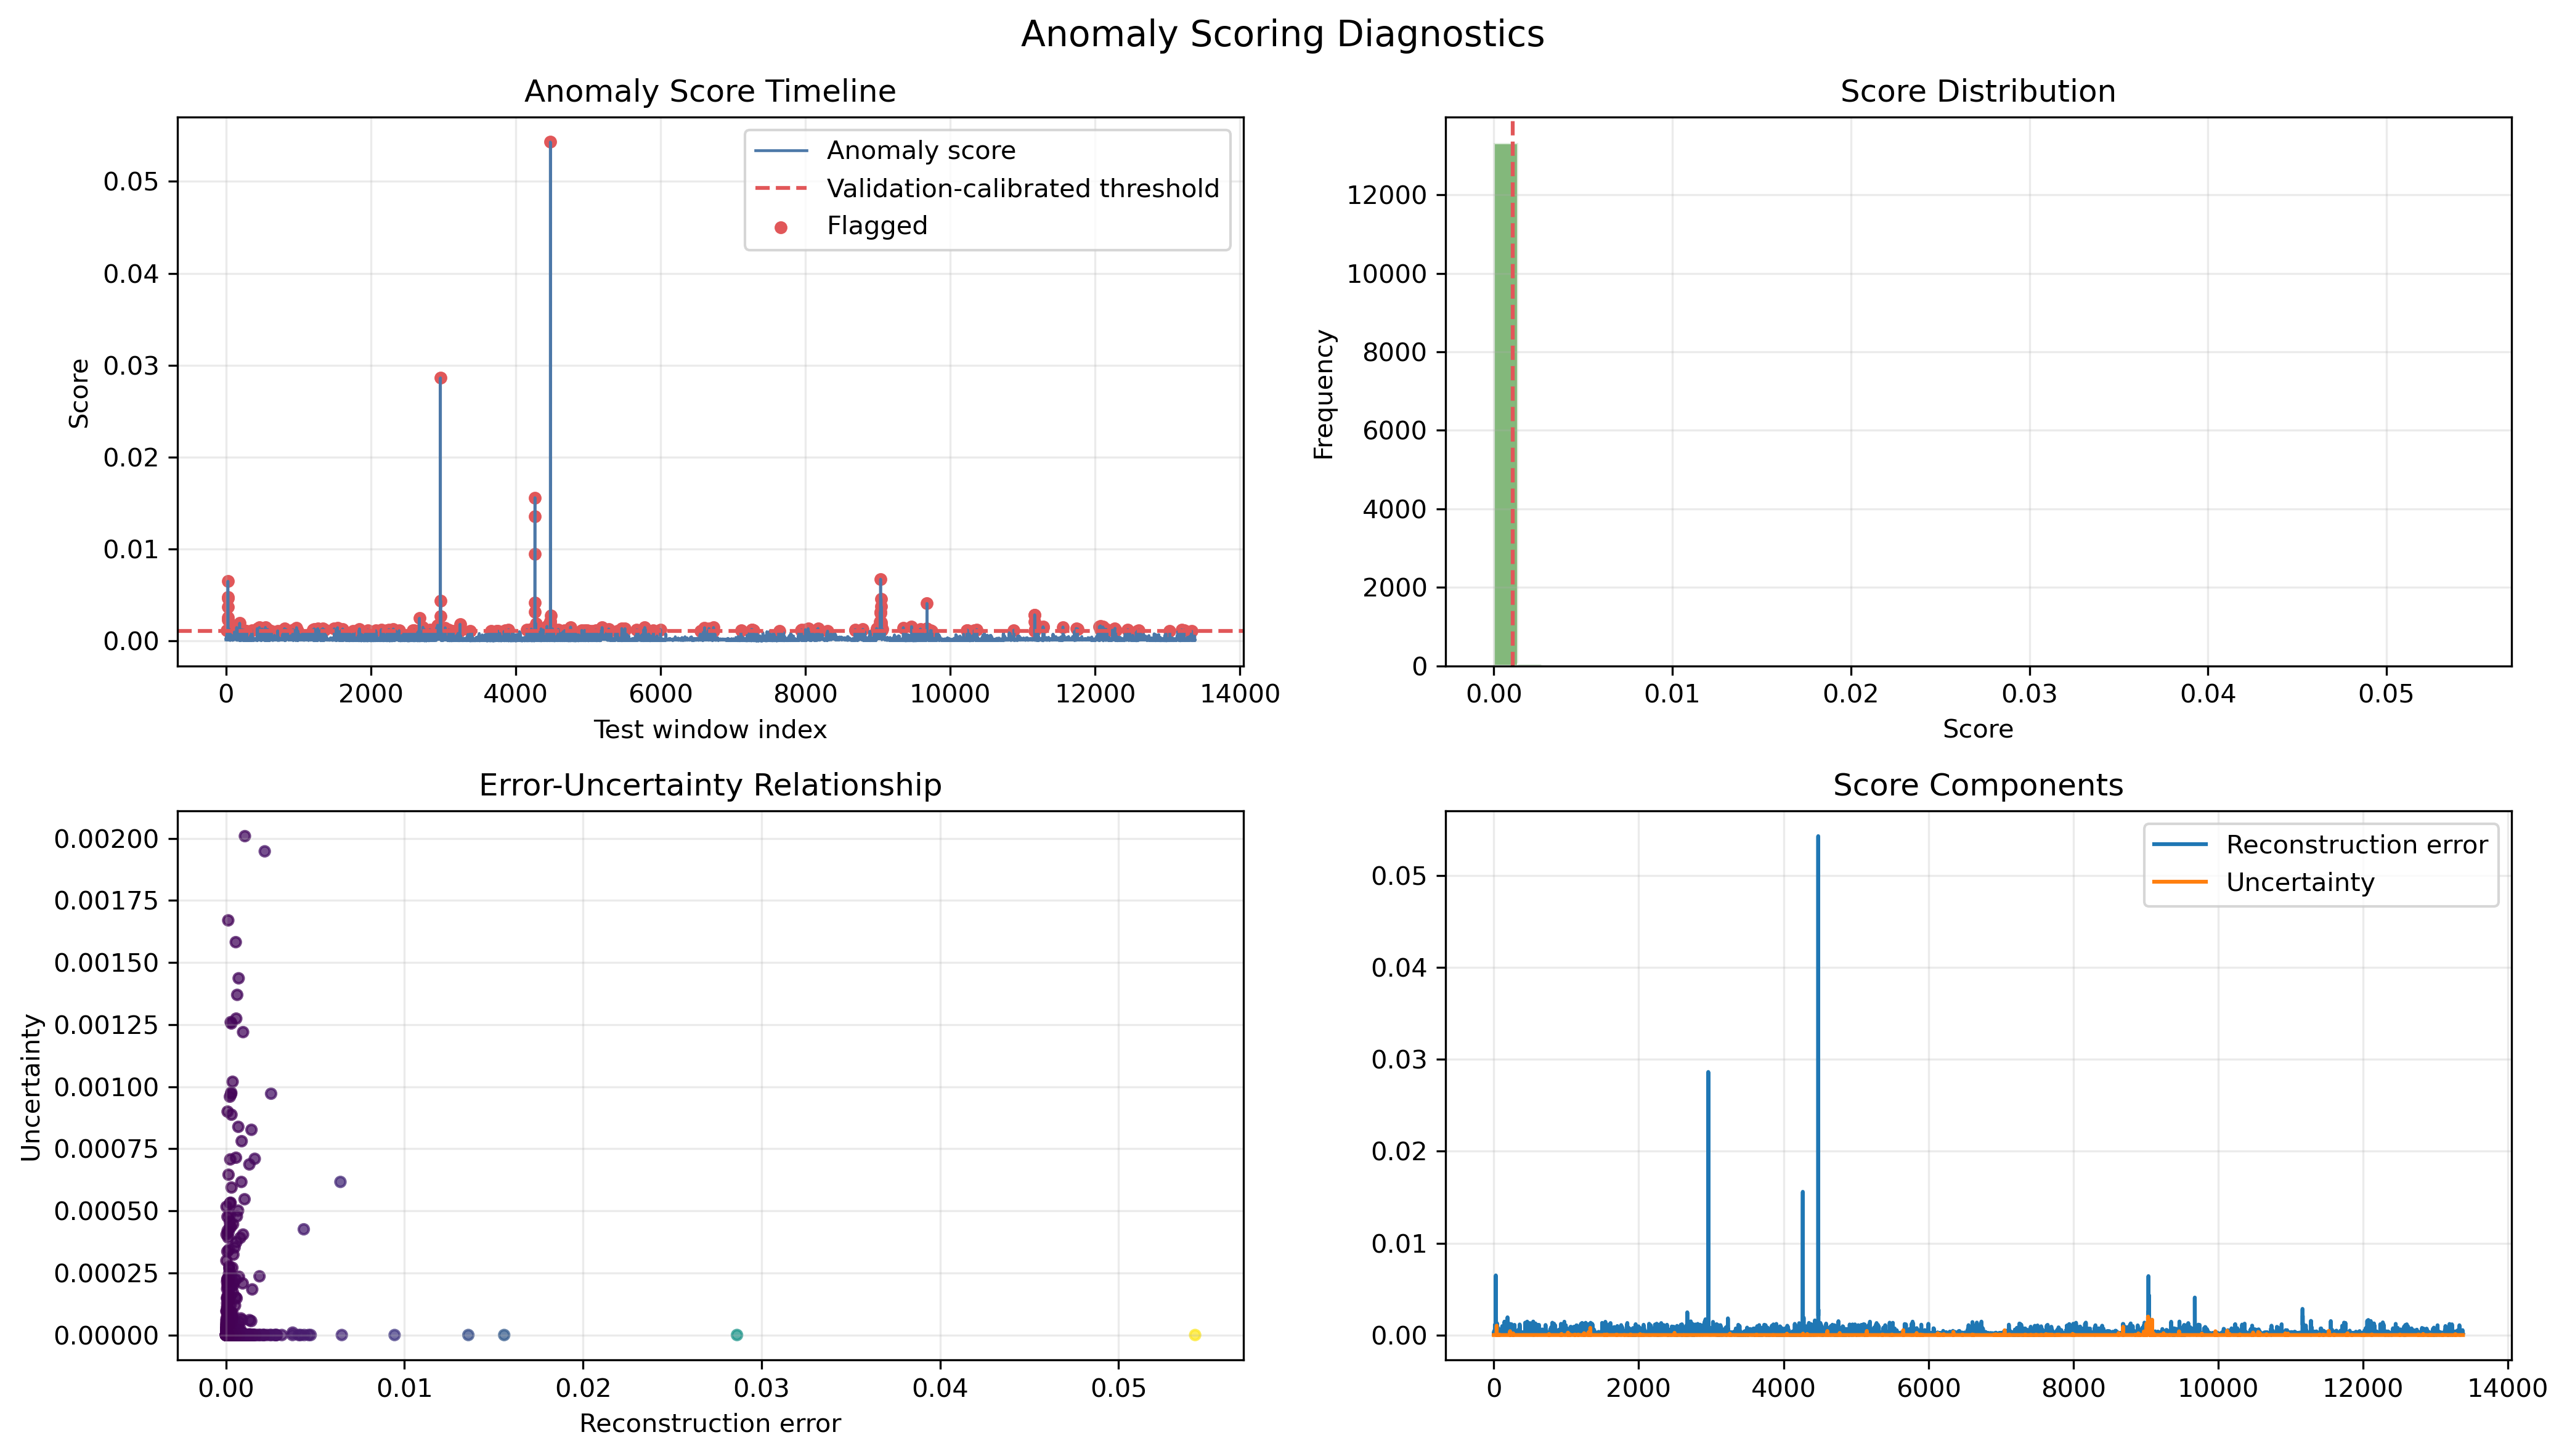
\includegraphics[width=\textwidth]{images/04_anomaly_diagnostics_base.png}\\[1pt]
{\small (a) Base TCN: $\tau_{95} = 1.06\times 10^{-3}$, 239 flagged (1.79\%).}\\[8pt]
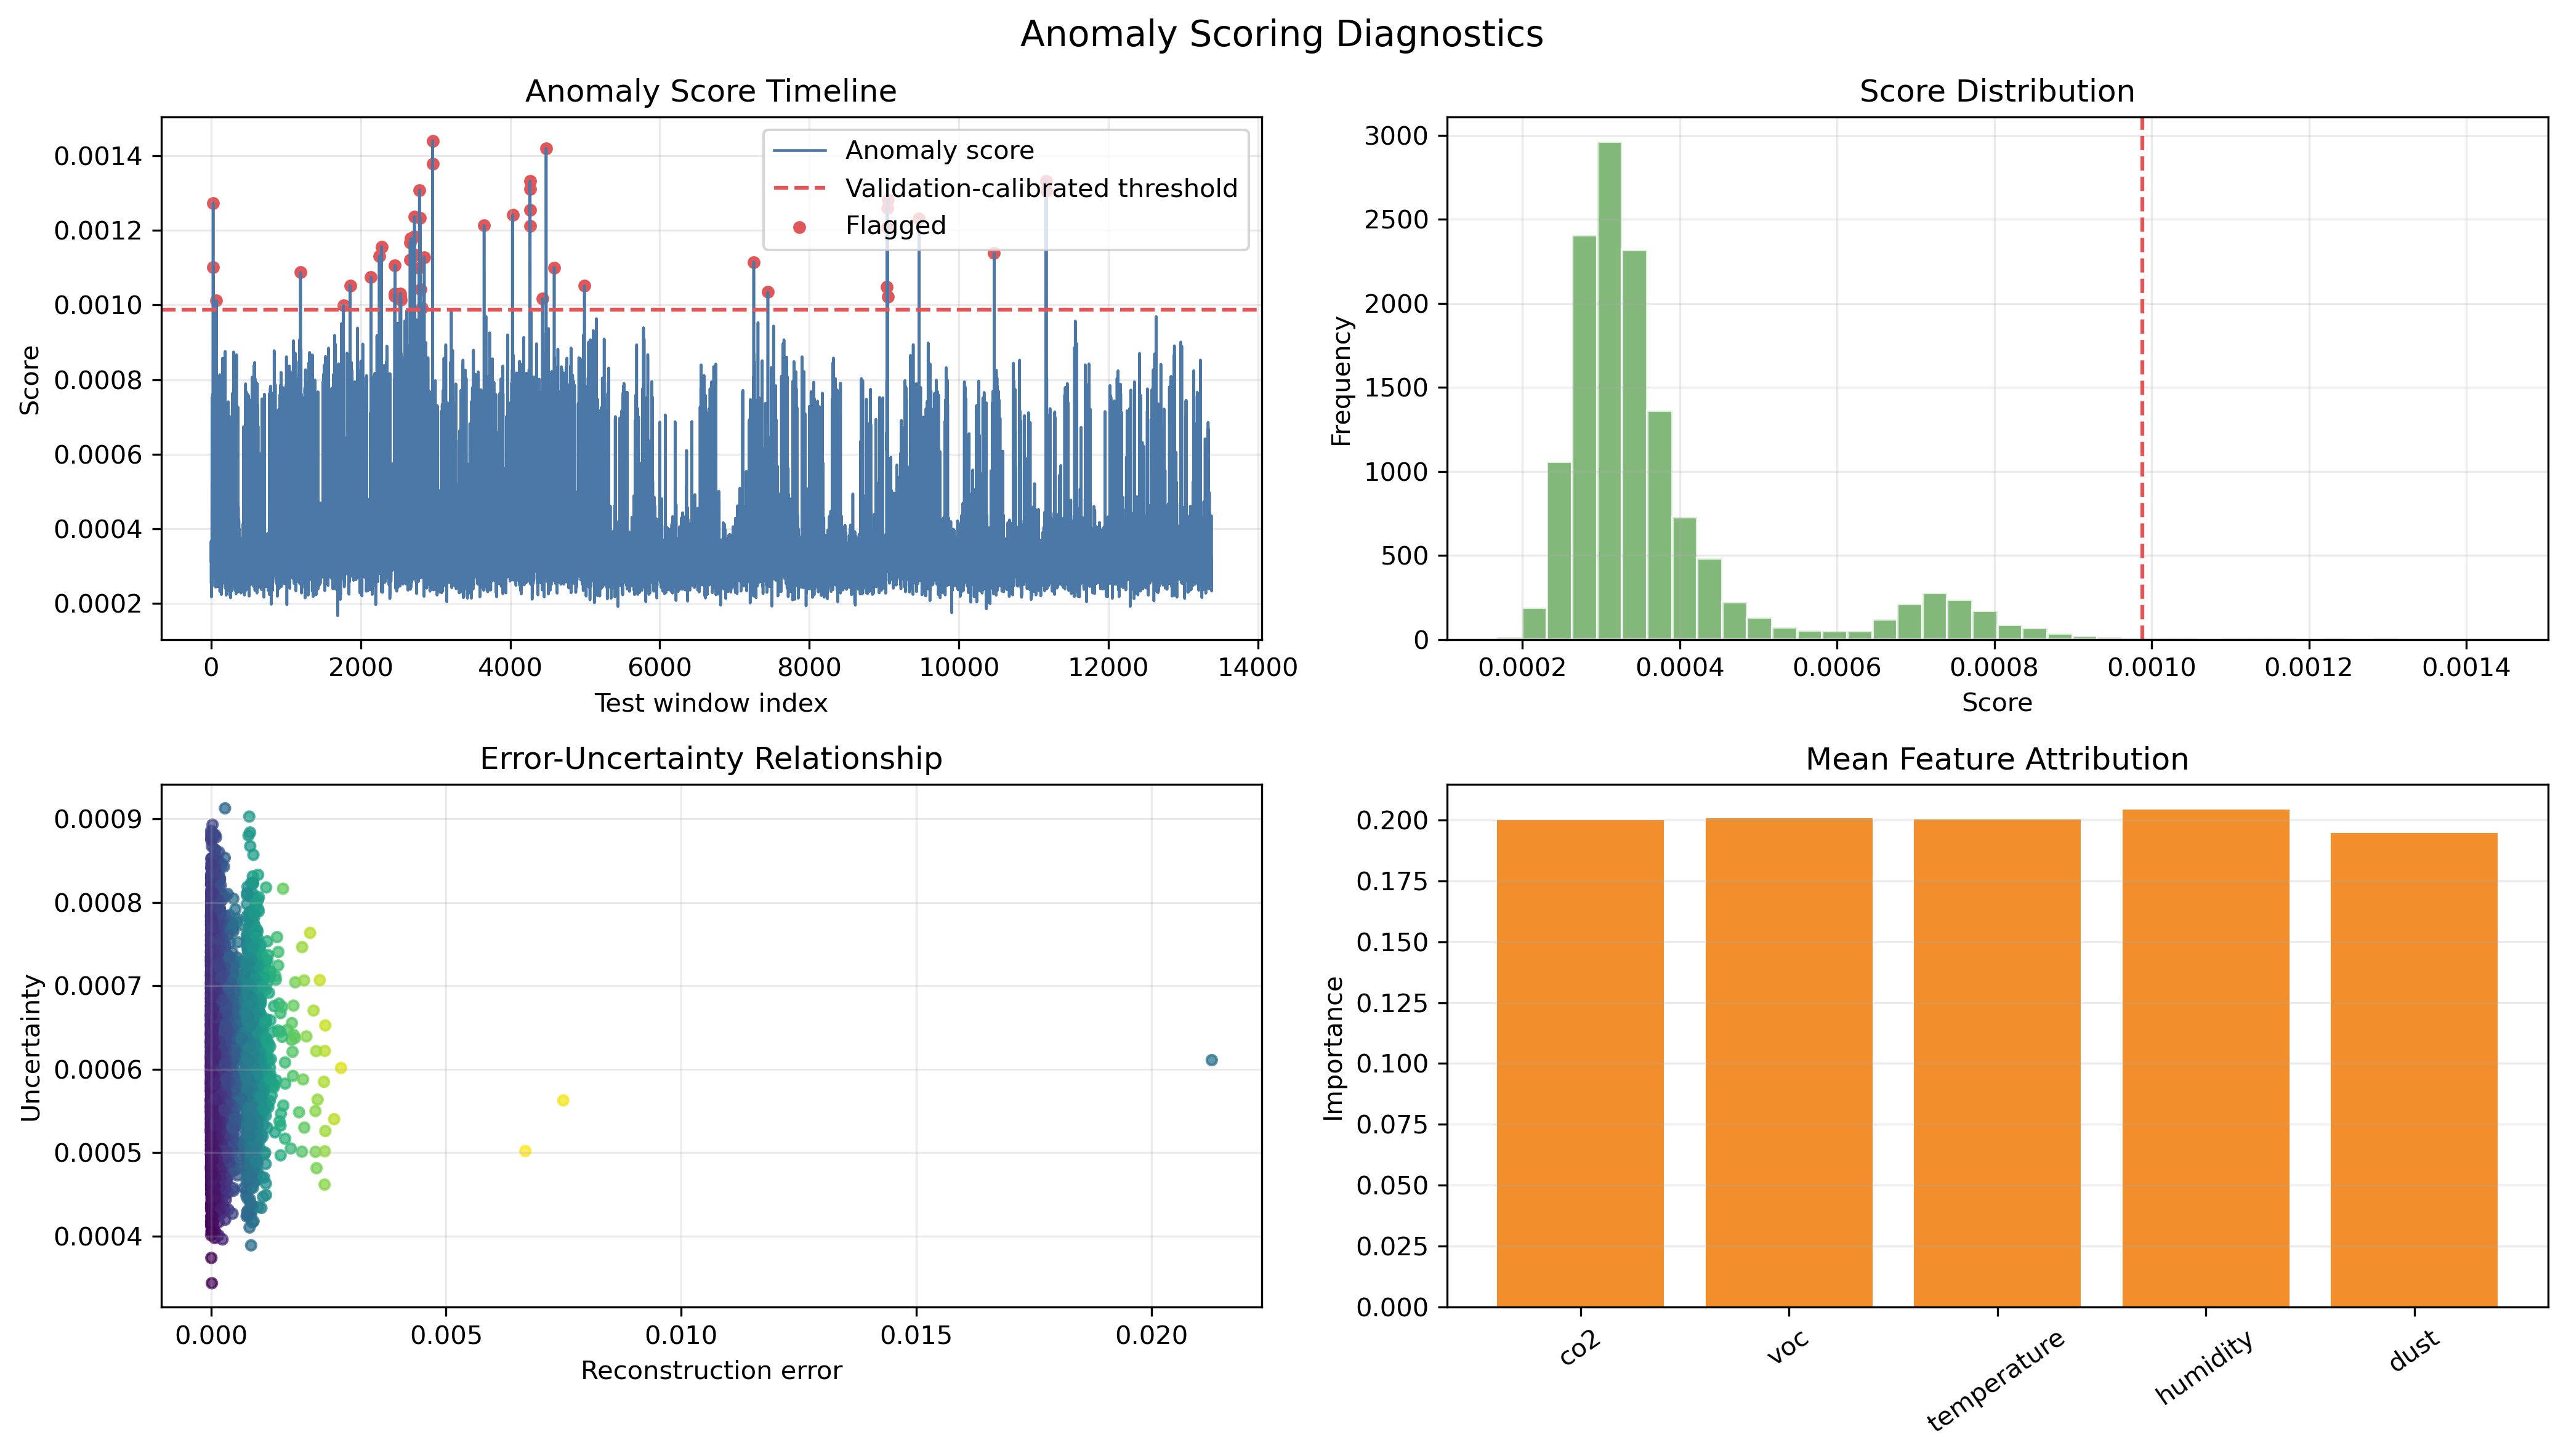
\includegraphics[width=\textwidth]{images/05_anomaly_diagnostics_enhanced.png}\\[1pt]
{\small (b) Full Enhanced (Proposed Model): $\tau_{95} = 9.93\times 10^{-4}$, 50 flagged (0.37\%).}
\caption{Anomaly detection diagnostics on the held-out test split for (a) Base TCN and (b) Full Enhanced, drawn with an identical four-panel layout and shared score axes for direct comparison: anomaly-score timeline (log $y$) with the validation-calibrated $\tau_{95}$ (dashed red) and flagged windows, score distribution (log $x$), error--uncertainty relationship (log--log), and per-sensor mean reconstruction error.}
\label{fig:anomaly_diagnostics}
\end{figure}

\subsection{Per-Sensor Attribution: Faithfulness Audit}

We treat the per-sensor attribution head as an \emph{exploratory} component and audit it rather than report it as a result. \cref{table:attribution} shows the attribution mass it assigns on the IAQ run---Humidity ($20.4\%$), VOC ($20.1\%$), CO\textsubscript{2} ($20.0\%$), Temperature ($20.0\%$), Dust ($19.5\%$)---which is essentially uniform. Such a flat distribution is not evidence that all sensors contribute equally; it is the signature of a head that fails to \emph{discriminate} among channels, as the audit below confirms.

\textbf{Controlled-perturbation faithfulness test.} We deliberately tested whether this near-uniform distribution reflects genuine per-sensor causal importance or merely an uninformative head, and we report the result candidly. On the labelled SKAB stream we ran a controlled-spike test: a $+6\sigma$ impulse was injected into one known channel of otherwise-normal windows, and we measured how often the learner's top-ranked channel matched the spiked one. The top-1 hit rate was only $0.127$, essentially at the random-chance level ($1/8 = 0.125$); the head collapses onto a single channel (it returned ``Voltage'' on $99.6\%$ of windows regardless of which channel was perturbed), and its attribution vector is not positively aligned with the per-channel reconstruction error on real anomalies (Spearman $\rho = -0.64$, $p = 0.09$). We therefore do \emph{not} claim that the attribution head provides validated, causally faithful explanations. The near-uniform IAQ distribution in \cref{table:attribution} should be read as the head failing to discriminate among channels rather than as evidence that all sensors contribute equally. We retain the module because it is trained jointly at negligible cost and the architecture supports attribution in principle, but making these attributions faithful (e.g.\ via gradient-based or perturbation-consistent attribution objectives) is an explicit direction for future work, not a present claim. The detection and uncertainty contributions of the framework do not depend on this head.

\begin{table}[H]
\centering
\caption{Attribution mass assigned by the feature-importance head on the IAQ run. The near-uniform distribution indicates the head does not discriminate among channels (see the faithfulness audit), and is reported as a diagnostic of this limitation rather than as a per-sensor importance result.}
\label{table:attribution}
\begin{tabular}{lc}
\toprule
\textbf{Sensor} & \textbf{Attribution} \\
\midrule
Humidity & 20.4\% \\
VOC & 20.1\% \\
CO\textsubscript{2} & 20.0\% \\
Temperature & 20.0\% \\
Dust (PM\textsubscript{2.5}) & 19.5\% \\
\bottomrule
\end{tabular}
\end{table}

\subsection{Additional Analyses}

\textbf{Computational Cost, Latency, and Scalability.} The Proposed model adds approximately 15\% more parameters relative to the Base TCN, primarily from the AUAA module (4 attention heads, 64-dim hidden) and the Dynamic Weight Adapter (context GRU, learned gating). \cref{table:latency_cost} reports measured inference cost on an NVIDIA GeForce GTX 1080 Ti with windows scored in a batch and the latency \emph{including} the full Monte-Carlo uncertainty pass. Per-window scoring latency scales linearly in $M$: $0.16$\,ms/window at the deployment budget $M=20$ and $0.29$\,ms/window at $M=50$, i.e.\ Monte-Carlo sampling is the dominant but still modest cost and is trivially parallel across the $M$ passes. A scalability probe over synthetic channel counts shows the convolutional backbone scales sub-linearly with the number of sensors, remaining under $1.2$\,ms/window up to $128$ channels. The principal cost driver for very high-rate or edge deployment is therefore the MC budget, which \cref{table:skab_msensitivity} shows can be reduced to $M=5$--$10$ with negligible detection loss; further reduction (single-pass distillation of the MC ensemble) is a natural edge-deployment route.

\begin{table}[H]
\centering
\caption{Measured inference cost (NVIDIA GeForce GTX 1080 Ti; latency includes the full Monte-Carlo pass). \textbf{Left:} per-window latency and F1 versus MC budget $M$ (8-channel SKAB). \textbf{Right:} per-window latency at $M=20$ versus sensor count $C$ (synthetic).}
\label{table:latency_cost}
\setlength{\tabcolsep}{8pt}\small
\begin{minipage}[t]{0.48\linewidth}\centering
\begin{tabular}{ccc}
\toprule
\textbf{$M$} & \textbf{ms/window} & \textbf{F1} \\
\midrule
5  & 0.023 & 0.476 \\
10 & 0.076 & 0.477 \\
20 & 0.162 & 0.477 \\
50 & 0.286 & 0.477 \\
\bottomrule
\end{tabular}
\end{minipage}\hfill
\begin{minipage}[t]{0.48\linewidth}\centering
\begin{tabular}{cc}
\toprule
\textbf{Channels $C$} & \textbf{ms/window ($M{=}20$)} \\
\midrule
8   & 1.06 \\
16  & 1.16 \\
32  & 0.76 \\
64  & 0.36 \\
128 & 0.37 \\
\bottomrule
\end{tabular}
\end{minipage}
\end{table}


\textbf{Robustness to sensor failures and noise.} Physical deployments suffer dropped sensor streams and noisy channels, so we stress-test the detector with its \emph{clean}-calibrated $\tau_{95}$ held fixed (\cref{table:skab_robustness}). Zeroing any single channel (a missing/failed stream) changes F1 by at most $0.006$, and injecting Gaussian noise up to $\sigma=1.0$ (standardized units) leaves F1 within $[0.475, 0.477]$. The multi-sensor fusion and uncertainty gating thus degrade gracefully rather than collapsing when an individual channel is corrupted. We did not test adversarial perturbations or inter-sensor time-synchronization errors; these remain open robustness questions for deployment.

\begin{table}[H]
\centering
\caption{Robustness on the SKAB test split with the clean-calibrated $\tau_{95}$ held fixed. Zeroing any single channel (a missing stream) or adding Gaussian noise up to $\sigma=1.0$ (standardized units) changes F1 by at most $0.006$.}
\label{table:skab_robustness}
\setlength{\tabcolsep}{7pt}\small
\begin{tabular}{lccc}
\toprule
\textbf{Condition} & \textbf{Precision} & \textbf{Recall} & \textbf{F1} \\
\midrule
Clean (reference)            & 0.556 & 0.417 & 0.477 \\
\midrule
Mask Accelerometer1RMS       & 0.556 & 0.417 & 0.477 \\
Mask Accelerometer2RMS       & 0.557 & 0.419 & 0.479 \\
Mask Current                 & 0.556 & 0.417 & 0.476 \\
Mask Voltage                 & 0.555 & 0.416 & 0.476 \\
Mask Pressure                & 0.556 & 0.418 & 0.477 \\
Mask Temperature             & 0.556 & 0.416 & 0.476 \\
Mask Thermocouple            & 0.556 & 0.416 & 0.476 \\
Mask Volume Flow RateRMS     & 0.555 & 0.426 & 0.482 \\
\midrule
Gaussian noise $\sigma=0.10$ & 0.556 & 0.416 & 0.476 \\
Gaussian noise $\sigma=0.25$ & 0.556 & 0.417 & 0.477 \\
Gaussian noise $\sigma=0.50$ & 0.555 & 0.416 & 0.475 \\
Gaussian noise $\sigma=1.00$ & 0.555 & 0.416 & 0.475 \\
\bottomrule
\end{tabular}
\end{table}


\textbf{Empirical calibration of the Chebyshev bound.} A distribution-free bound is only useful if it is respected in practice and not vacuously loose. \cref{table:chebyshev_calib} reports, on the SKAB normal validation windows, the observed false-positive rate at $\tau=\bar{s}+k\sigma_s$ against the guarantee $1/k^2$. The empirical rate stays below the bound at every $k$ (e.g.\ at the design point $k=4.47$ the bound is $0.05$ and the observed rate is $0.000$). On this corpus the score distribution is close to Gaussian (skewness $-0.23$, excess kurtosis $0.11$), so the bound is conservative, yet it remains the correct tool precisely because it stays valid without distributional assumptions: under the heavy-tailed or skewed score distributions that arise on other sensor corpora the Gaussian/percentile thresholds lose their coverage guarantee while the Chebyshev threshold does not. We therefore present it as a safe \emph{worst-case} operating point to be used alongside, not instead of, the empirical percentile threshold.

\begin{table}[H]
\centering
\caption{Empirical validation of the Chebyshev false-positive bound on the SKAB clean validation windows ($n=6190$). The observed false-positive rate at $\tau=\bar{s}+k\sigma_s$ stays below the distribution-free guarantee $1/k^2$ at every $k$.}
\label{table:chebyshev_calib}
\setlength{\tabcolsep}{8pt}\small
\begin{tabular}{ccc}
\toprule
\textbf{$k$} & \textbf{Bound $1/k^2$} & \textbf{Empirical FP rate} \\
\midrule
1.00 & 1.0000 & 0.15283 \\
1.50 & 0.4444 & 0.05945 \\
2.00 & 0.2500 & 0.01858 \\
3.00 & 0.1111 & 0.00032 \\
4.00 & 0.0625 & 0.00000 \\
4.47 & 0.0500 & 0.00000 \\
5.00 & 0.0400 & 0.00000 \\
\bottomrule
\end{tabular}
\end{table}


\textbf{Choice of uncertainty estimator.} MC dropout is one of several uncertainty-quantification options. To check that it is not a limiting choice, we compared it against a five-member deep ensemble of the forecaster under the identical hybrid-scoring protocol: the ensemble reaches F1 $0.110$ / ROC-AUC $0.685$ on SKAB, comparable to the single-model MC-dropout detector at the same (Base-TCN) architecture level (Base TCN, F1 $0.113$), while requiring $5\times$ the training and storage. This indicates that the detection gains in our framework come from the uncertainty-\emph{aware architecture} (AUAA and the dynamic weight adapter), not from the particular uncertainty estimator, and that MC dropout is the cost-efficient choice (a single model, $M$ trivially-parallel passes). Variational inference and evidential heads would require architectural changes and are known to be calibration-sensitive, while conformal prediction is complementary and is already reflected in our distribution-free Chebyshev threshold; we leave a full estimator sweep to future work.

\textbf{MC Sample Sensitivity.} The full evaluation reported above uses $M=50$ Monte Carlo samples; the sensitivity table in \cref{table:mc_sensitivity} reports indicative MSE values at smaller $M$ obtained by drawing the first $M$ samples from the same ensemble. Performance converges around $M \approx 20$, beyond which marginal gains plateau while computational cost scales linearly. For operational deployment with a 1-minute sensor sampling cycle we recommend $M=20$ (per-batch latency $<30$~ms), and $M=50$ for offline evaluation where calibration is the priority.

To confirm that this two-budget choice does not affect the \emph{detection} conclusions, \cref{table:skab_msensitivity} re-runs the SKAB evaluation at $M\in\{5,10,20,50\}$ and reports precision/recall/F1/ROC-AUC. The proposed model's F1 is essentially invariant ($0.476$--$0.477$ across all $M$) and its ROC-AUC rises by only $0.003$ from $M=20$ to $M=50$; the deployment budget $M=20$ therefore incurs no meaningful detection penalty. We use $M=50$ for the IAQ \emph{forecasting/calibration} numbers (where the predictive variance enters the uncertainty-calibration loss and the reliability diagram) and $M=20$ for the deployment-faithful detection benchmark; \cref{table:skab_msensitivity} shows the two budgets are interchangeable for detection, so the choice is one of latency rather than accuracy.

\begin{table}[H]
\centering
\caption{SKAB detection metrics versus the Monte-Carlo budget $M$ (seed 42, validation-calibrated $\tau_{95}$). F1 is essentially invariant to $M$ and ROC-AUC rises only $+0.003$ from $M=20$ to $M=50$.}
\label{table:skab_msensitivity}
\setlength{\tabcolsep}{6pt}\small
\begin{tabular}{lcccc}
\toprule
 & \multicolumn{2}{c}{\textbf{Base TCN}} & \multicolumn{2}{c}{\textbf{Full Enhanced}} \\
\cmidrule(lr){2-3}\cmidrule(lr){4-5}
\textbf{$M$} & \textbf{F1} & \textbf{ROC-AUC} & \textbf{F1} & \textbf{ROC-AUC} \\
\midrule
5  & 0.046 & 0.676 & 0.476 & 0.723 \\
10 & 0.063 & 0.677 & 0.477 & 0.725 \\
20 & 0.054 & 0.678 & \textbf{0.477} & 0.727 \\
50 & 0.061 & 0.679 & 0.477 & 0.730 \\
\bottomrule
\end{tabular}
\end{table}


\begin{table}[H]
\centering
\caption{Monte Carlo sample-count sensitivity of the Full Enhanced model's forecasting MSE and $R^2$ on the held-out \textbf{IAQ} test split (truncated subsets of the same $M=50$ ensemble; relative-time figures are forward-pass cost scaled with $M$).}
\label{table:mc_sensitivity}
\begin{tabular}{lccc}
\toprule
\textbf{$M$ Samples} & \textbf{MSE} & \textbf{R\textsuperscript{2}} & \textbf{Relative time} \\
\midrule
5   & $1.85\times 10^{-4}$ & 0.9986 & 0.10$\times$ \\
10  & $1.74\times 10^{-4}$ & 0.9987 & 0.20$\times$ \\
20  & $1.68\times 10^{-4}$ & 0.9988 & 0.40$\times$ \\
50  & $1.65\times 10^{-4}$ & 0.9988 & 1.00$\times$ \\
\bottomrule
\end{tabular}
\end{table}

\textbf{Threshold Comparison.} Three threshold methods produce different operating points on the test set with validation-calibrated parameters. The percentile method yields $\tau_{95} = 1.06\times 10^{-3}$ for the Base model and $\tau_{95} = 9.93\times 10^{-4}$ for the Proposed model. The adaptive threshold $\tau_{\text{adapt}} = \tau_{\text{base}} \cdot (0.8 + 0.4\bar{\alpha})$ with $\bar{\alpha} = 0.527$ produces a slightly higher operating point ($1.07\times 10^{-3}$ and $1.00\times 10^{-3}$ respectively). The Chebyshev threshold with $k = \sqrt{1/0.05} \approx 4.47$ provides distribution-free FP-rate control with the guarantee $P(\text{FP}) \leq 1/k^2 = 0.05$. The Chebyshev bound is conservative (no Gaussian assumption is made on the score distribution), offering a principled operating point for safety-critical deployments where false alarms carry high operational cost.

% ============================================================
\section{Discussion}

\subsection{Interpretation of Results}

The ablation results provide direct evidence for the role of auxiliary objectives in shaping the encoder representation. Adding MC dropout to the deterministic Base TCN leaves point-prediction MSE essentially unchanged ($+0.005\%$), confirming that MC dropout's primary contribution is uncertainty estimation rather than forecasting improvement. Activating the dynamic-weight regularizer and the feature-attribution loss together (without AUAA) produces the largest single jump in MSE ($-26.25\%$), demonstrating that the composite objective itself not merely model capacity drives the reduction. Adding AUAA on top of the auxiliary objectives produces near-equivalent MSE ($-25.19\%$): AUAA's contribution is therefore most visible in \emph{anomaly scoring} (uncertainty-gated attention re-weights time steps with high $\sigma_t$) rather than in forecasting metrics that average over time.

The dynamic weight adapter's central tendency $\bar{\alpha} = 0.527$ on the test split sits slightly above $0.5$, indicating mild bias toward reconstruction error in this indoor-air-quality regime. The observed range $\alpha \in [0.003, 0.537]$ confirms that the gating module remains responsive: a small subset of windows triggers near-zero $\alpha$ (uncertainty-dominated scoring) while the dominant operating mode lies near the central tendency. The adapter learns this context dependence end-to-end without manual threshold tuning.

\subsection{Comparison with Prior Stochastic TCN Frameworks}

Our framework extends stochastic TCNs along three architectural dimensions. First, \textbf{uncertainty integration depth}: prior work~\cite{ghimire_electricity_2025, cui_sde-hnn_2025} applies uncertainty post hoc as a scoring term, while our AUAA feeds it into attention computation, consistent with the epistemic/aleatoric decomposition formalized by Kendall and Gal~\cite{kendall2017uncertainties}. Second, \textbf{adaptive vs.\ fixed scoring}: our dynamic weight adapter replaces static $\alpha$ with a context-sensitive mechanism. Third, \textbf{explanatory ambition}: the framework includes a per-sensor attribution head, although our audit (Section~4.7) shows it is not yet causally faithful, so we present it as an exploratory component rather than a delivered capability over prior frameworks~\cite{audibert2020usad, malhotra2016lstmed, zhao2020mtadgat}. The cross-dataset improvement on SKAB ($8.8\times$ F1, $14.4\times$ recall over the Base TCN; \cref{sec:skab_cross_dataset}) confirms that these architectural differences yield measurable gains beyond the IAQ domain. Benchmarked against twelve established detectors under a single unified protocol (\cref{table:skab_baselines}), the proposed model attains the best F1 and the best recall of the panel, while the strongest reconstruction baselines retain higher precision and a marginally higher ROC-AUC. We therefore position the contribution honestly: it is a \emph{recall-oriented} detector whose advantage is the recovery of slow, partial fault signatures that reconstruction-only methods miss, rather than a method that uniformly dominates every metric.

Against the broader families the reviewer raises, the novelty is one of \emph{integration} rather than a new estimator or backbone. Bayesian/stochastic TCNs~\cite{ghimire_electricity_2025, cui_sde-hnn_2025} and uncertainty-aware transformers attach predictive uncertainty as an output-level scoring term; graph-based detectors (MTAD-GAT~\cite{zhao2020mtadgat}) model inter-sensor structure but not reliability; and interpretable industrial monitors add post-hoc explanations. Our framework instead routes the MC-dropout uncertainty \emph{back into} the computation---gating attention (AUAA) and conditioning a learned reconstruction/uncertainty blend (Dynamic Weight Adapter)---and pairs it with a distribution-free operating guarantee. The empirical value of this integration, rather than of the uncertainty estimator itself, is established in two ways above: the deep-ensemble comparison shows the estimator choice is not the source of the gain, and the unified twelve-method benchmark (\cref{table:skab_baselines}) shows the integrated model leads on F1/recall. The positioning of \cref{table:positioning} summarizes which of these four properties---uncertainty quantification, adaptive attention, sensor adaptation, and feature attribution---each family provides.

\subsection{Uncertainty Calibration}

Qualitatively, MC dropout uncertainty estimates tracked prediction difficulty: uncertainty increased during rapid environmental transitions (morning ventilation onset, occupancy changes) and decreased during stable nighttime periods. \cref{fig:uncertainty_calibration} reports the reliability diagram on the test split (left) alongside the distribution of predictive standard deviations (right). The reliability diagram shows that the model's calibrated predictive intervals are mildly \emph{conservative}: empirical coverage sits above the diagonal at low-to-moderate nominal confidence (intervals slightly wider than required) and converges to near-perfect calibration at the high-confidence levels relevant for alarms (empirical coverage $\approx 0.95$ at the $95\%$ nominal level). The raw MC-dropout epistemic standard deviation $\boldsymbol{\sigma}_t$ shown in panel~(b) (mean $\bar{\sigma}=6.18\times 10^{-4}$) is only the epistemic component and is necessarily narrower; the calibrated interval used for the reliability curve combines it with the learned variance head. In either case the distribution-free Chebyshev bound used for threshold selection (Section 3.6) provides the deployment-time FP-rate guarantee independently of this calibration profile. The architectural integration of uncertainty distinguishes this work from standalone calibration studies~\cite{gal2016dropout_bayesian, lakshminarayanan2017ensembles}.

\begin{figure}[H]
\centering
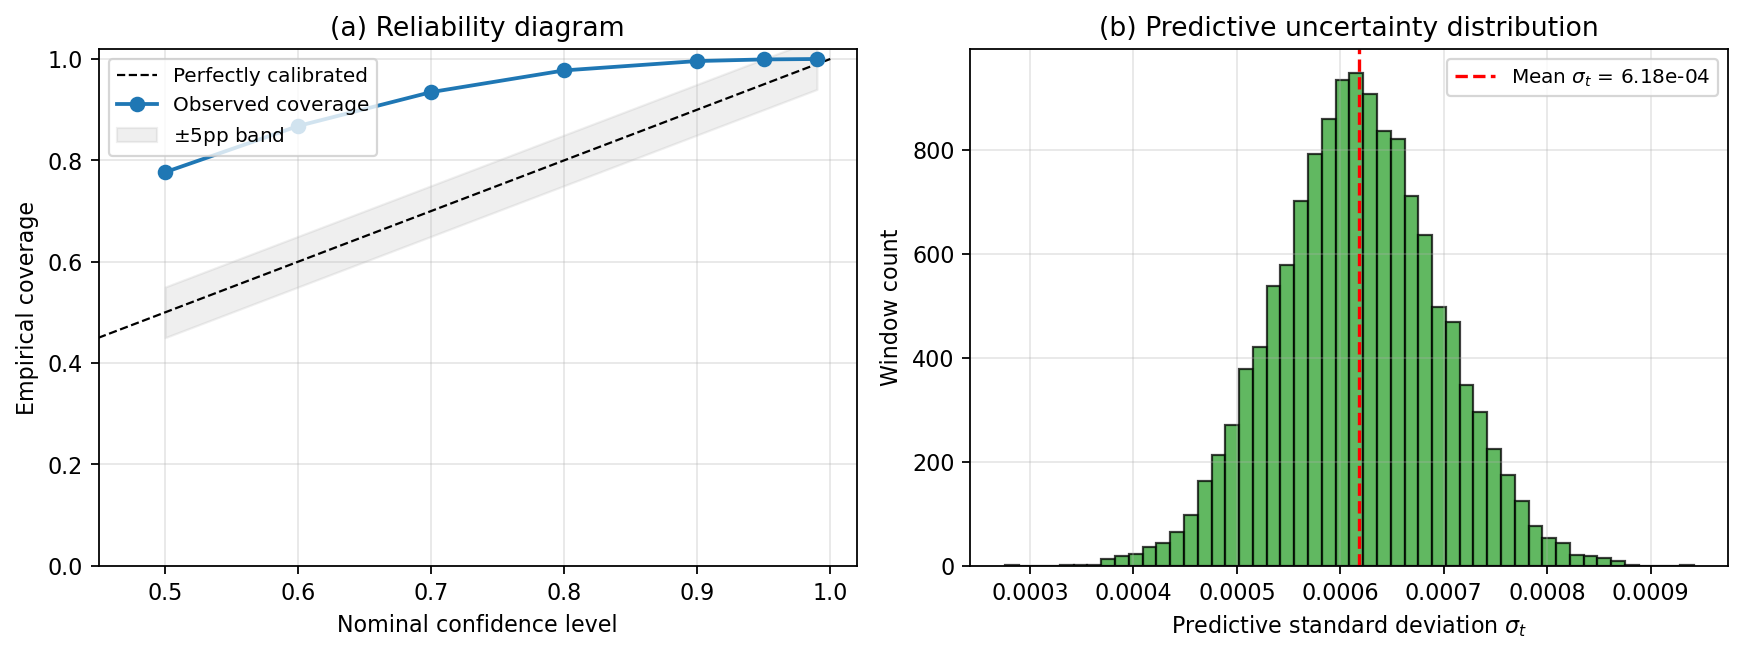
\includegraphics[width=\textwidth]{images/08_uncertainty_calibration.png}
\caption{Uncertainty calibration on the held-out test split. \textbf{(a)} Reliability diagram (empirical coverage vs.\ nominal confidence; the diagonal is perfect calibration, below it is over-confidence). \textbf{(b)} Histogram of per-window predictive standard deviation $\boldsymbol{\sigma}_t$ ($M=50$), centred at $\bar{\sigma} = 6.18\times 10^{-4}$.}
\label{fig:uncertainty_calibration}
\end{figure}

\subsection{Sensor-Specific Design Justification}

Each architectural choice is motivated by a concrete sensor-characteristic argument:

\textbf{AUAA justified by sensor heterogeneity.} The uncertainty gate $1/(1 + \sigma_t)$ is motivated by the observation that sensor noise variance varies both across sensor types (e.g., electrochemical VOC vs.~thermistor temperature) and over time (sensor aging, environmental interference). A mechanism that uniformly treats all attention positions is suboptimal when some positions carry substantially more reliable information than others.

\textbf{Dynamic weighting justified by sensor degradation.} Fixed-weight scoring implicitly assumes constant sensor quality—an assumption violated by real sensor deployments where CO\textsubscript{2} sensor drift and VOC sensitivity degradation evolve on timescales of days to weeks. The dynamic adapter's GRU state provides memory of recent sensor behavior, enabling adaptation to degradation trends.

\textbf{Attribution justified by maintenance workflows.} In facility management, an anomaly attributed to CO\textsubscript{2} triggers HVAC inspection, while one attributed to dust triggers filter replacement—different sensor attributions lead to different operational responses. The attribution head is intended to provide this sensor-level granularity; we include it for this reason but, per the faithfulness audit (Section~4.7), it does not yet do so reliably and is reported as a limitation rather than a solved capability.

\subsection{Design Extensions and Deployment Considerations}

The sensor-specific design principles established in this work suggest natural extensions. Training under normal-operation assumptions means contamination by undetected anomalies can bias predictive distributions, robust training strategies such as trimmed loss functions offer a direct mitigation path. The current single-step prediction scope can be extended to multi-horizon forecasting using long-context Transformer variants such as Informer~\cite{zhou2021informer} or TimesNet~\cite{wu2022timesnet} for detecting gradual drift patterns that emerge over longer timescales. Graph-attention extensions such as MTAD-GAT~\cite{zhao2020mtadgat} provide a path for modelling explicit inter-sensor dependencies that the current channel-independent architecture does not capture. For higher-frequency sensor streams (e.g., 100~Hz vibration monitoring), model distillation or reducing the number of MC samples allows architectural benefits to be preserved within tighter latency constraints. Assumptions regarding a fixed sensor set can be relaxed through dynamic input filtering, and online learning variants can address conceptual shifts in non-stationary environments.

\subsection{Limitations}

We state the boundaries of the present study explicitly. \textbf{(i) Attribution faithfulness.} The feature-importance head is not yet causally faithful: under a controlled $+6\sigma$ single-channel spike its top-ranked channel matches the perturbed one only $12.7\%$ of the time (chance $12.5\%$) and it collapses onto a single channel, so we report it as an architectural placeholder and a future-work target rather than a validated explanation (Section~4.7). \textbf{(ii) Effect size.} The IAQ forecasting gain, while statistically significant (Section~4.3), is modest in absolute MSE; we have accordingly reframed the contribution around detection recall and operational guarantees rather than headline accuracy, and we avoid claiming large forecasting improvements. \textbf{(iii) Component interactions.} The ablation (\cref{table:ablation}) varies components cumulatively and shows no negative interaction, but it is not a full $2^3$ factorial, so synergy versus independence among AUAA, the dynamic adapter, and the attribution head is only partially resolved. \textbf{(iv) Domain coverage.} Both evaluation domains (indoor air quality and industrial water circulation) are comparatively stationary; generalization to highly non-stationary or heterogeneous cyber-physical streams, and robustness to adversarial perturbations and inter-sensor synchronization errors (beyond the channel-masking and Gaussian-noise tests of Section~4.8), remain open. \textbf{(v) Theoretical scope.} The Monte-Carlo convergence result (\cref{thm:mc_convergence}) is a standard SLLN/CLT consequence repurposed here to justify the sample budget $M$ rather than a new probabilistic result; its role is to make the $O(M^{-1/2})$ trade-off explicit, and the Chebyshev bound, though valid and empirically respected (\cref{table:chebyshev_calib}), is intentionally conservative for near-Gaussian scores.

\section{Conclusions}

We introduced an uncertainty-aware TCN framework that treats predictive uncertainty as an internal architectural signal rather than a post-hoc add-on, accompanied by two distribution-free theoretical guarantees that anchor the operational pipeline. The framework is motivated by three sensor-specific challenges, heterogeneous reliability drift across sensor types, context-dependent anomaly scoring requirements, and the need for actionable per-sensor diagnostic output---and integrates two uncertainty-driven components: (1) the Adaptive Uncertainty-Aware Attention (AUAA) mechanism gates temporal attention by per-sensor predictive uncertainty from MC dropout; and (2) the Dynamic Weight Adapter learns context-sensitive blending of reconstruction error and uncertainty. The Chebyshev-type bound (\cref{thm:chebyshev_fp}) furnishes a distribution-free false-positive guarantee on the hybrid score, and the Monte-Carlo convergence result (\cref{thm:mc_convergence}) sets the sample-size budget $M$ for the inference pass. The architecture also includes a per-sensor attribution head, but we audit it rather than claim it as a result.

Comprehensive experiments on four-month IAQ sensor data demonstrated a $25.2\%$ MSE reduction on the held-out test split (Base $2.20\times 10^{-4}$ vs.\ Full Enhanced $1.65\times 10^{-4}$; $R^2$ 0.9988, SMAPE 11.07\%). The ablation isolates the source of this gain: the auxiliary objectives (dynamic-weight regularizer and feature-attribution loss) deliver the dominant reduction, while AUAA contributes uncertainty-gated attention at scoring time without further reducing forecasting MSE. A cross-dataset validation on the Skoltech Anomaly Benchmark (\cref{sec:skab_cross_dataset}) supplies independent, third-party ground-truth labels and confirms that the Full Enhanced configuration recovers a $7.7\times$ higher F1 ($0.477$ vs.\ $0.062$) and $12.6\times$ higher recall ($0.418$ vs.\ $0.033$) than the Base TCN on a domain (industrial water-circulation sensors) disjoint from the IAQ training distribution. The architecture additionally produces a per-sensor attribution output, although a controlled-perturbation audit (Section~4.7) shows this head is not yet causally faithful---we report it transparently as a limitation and future-work target rather than a validated explanation. The Chebyshev bound of \cref{thm:chebyshev_fp} guarantees $P(\text{FP}) \leq 1/k^2$ without distributional assumptions and is empirically respected on the benchmark. With sub-millisecond per-window inference ($0.16$\,ms at $M=20$, including the uncertainty pass) and $\sim 15\%$ parameter overhead, the framework is suitable for real-time deployment in smart buildings, environmental monitoring, and industrial process control.

\vspace{6pt}
\noindent\textbf{Operational Guarantee:} Applying the Chebyshev inequality to anomaly score distributions yields a distribution-free false-positive-rate bound: for any score distribution with finite variance and threshold \(\tau = \bar{s} + k \cdot \sigma_s\), the detector satisfies \(P(\text{FP}) \leq 1/k^2\). This enables principled threshold selection without parametric distributional assumptions, providing an operational guarantee that complements the empirical percentile-based approach.

% === BACK MATTER ===
\authorcontributions{Conceptualization, V.P.W. and C.S.K.; methodology, V.P.W.; software, V.P.W.; validation, V.P.W., K.H.R., I.F and C.S.K.; formal analysis, V.P.W. and I.F; investigation, V.P.W.; resources, C.S.K., Y.P.H; data curation, V.P.W.; writing---original draft preparation, V.P.W.; writing---review and editing, K.H.R. and C.S.K.; visualization, V.P.W., I.F; supervision, K.H.R., C.S.K., Y.P.H; project administration, C.S.K.; funding acquisition, C.S.K., K.H.R}

\funding{This study was funded and conducted with the support of the RealSecu Small and Medium Business Technology Innovation Development (R\&D) project 'AI, Security Solution to Block the Leakage of Internal Confidential Information through Machine Learning' (RS-2024-00514290) and by the Basic Science Research Program through the National Research Foundation of Korea (NRF), funded by the Ministry of Education (2021R1I1A3052605).}

\institutionalreview{Not applicable.}
\informedconsent{Not applicable.}
\dataavailability{The dataset is publicly accessible: the raw (pre-filtering) recording at \url{https://raw.githubusercontent.com/vandhapw/datasets/refs/heads/main/filtered_data.csv} and the DBSCAN-filtered data used for modelling at \url{https://raw.githubusercontent.com/vandhapw/datasets/refs/heads/main/df_normal.csv}.}

\conflictsofinterest{The authors declare no conflicts of interest.}

% \clearpage
\reftitle{References}
% \bibliography{2209-hiper-chad}
\bibliography{corrected_references}

\end{document}
